 

% Slides for FYS4480


\documentclass[compress]{beamer}


% Try the class options [notes], [notes=only], [trans], [handout],
% [red], [compress], [draft], [class=article] and see what happens!

% For a green structure color use:
%\colorlet{structure}{green!50!black}

\mode<article> % only for the article version
{
  \usepackage{beamerbasearticle}
  \usepackage{fullpage}
  \usepackage{hyperref}
}

\beamertemplateshadingbackground{red!10}{blue!10}

%\beamertemplateshadingbackground{red!10}{blue!10}
\beamertemplatetransparentcovereddynamic
%\usetheme{Hannover}

\setbeamertemplate{footline}[page number]


%\usepackage{beamerthemeshadow}

%\usepackage{beamerthemeshadow}
\usepackage{ucs}


\usepackage{pgf,pgfarrows,pgfnodes,pgfautomata,pgfheaps,pgfshade}
\usepackage{graphicx}
\usepackage{simplewick}
\usepackage{amsmath,amssymb}
\usepackage[latin1]{inputenc}
\usepackage{colortbl}
\usepackage[english]{babel}
\usepackage{listings}
\usepackage{shadow}
\lstset{language=c++}
\lstset{alsolanguage=[90]Fortran}
\lstset{basicstyle=\small}
%\lstset{backgroundcolor=\color{white}}
%\lstset{frame=single}
\lstset{stringstyle=\ttfamily}
%\lstset{keywordstyle=\color{red}\bfseries}
%\lstset{commentstyle=\itshape\color{blue}}
\lstset{showspaces=false}
\lstset{showstringspaces=false}
\lstset{showtabs=false}
\lstset{breaklines}
\usepackage{times}

% Use some nice templates
\beamertemplatetransparentcovereddynamic

% own commands
\newcommand*{\cre}[1]{a^{\dagger}_{#1}}
\newcommand*{\an}[1]{a_{#1}}
\newcommand*{\crequasi}[1]{b^{\dagger}_{#1}}
\newcommand*{\anquasi}[1]{b_{#1}}
\newcommand*{\for}[3]{\langle#1|#2|#3\rangle}
\newcommand{\be}{\begin{equation}}
\newcommand{\ee}{\end{equation}}
\newcommand*{\kpr}[1]{\left\{#1\right\}}
\newcommand*{\ket}[1]{|#1\rangle}
\newcommand*{\bra}[1]{\langle#1|}
%\newcommand{\bra}[1]{\left\langle #1 \right|}
%\newcommand{\ket}[1]{\left| # \right\rangle}
\newcommand{\braket}[2]{\left\langle #1 \right| #2 \right\rangle}
\newcommand{\OP}[1]{{\bf\widehat{#1}}}
\newcommand{\matr}[1]{{\bf \cal{#1}}}
\newcommand{\beN}{\begin{equation*}}
\newcommand{\bea}{\begin{eqnarray}}
\newcommand{\beaN}{\begin{eqnarray*}}
\newcommand{\eeN}{\end{equation*}}
\newcommand{\eea}{\end{eqnarray}}
\newcommand{\eeaN}{\end{eqnarray*}}
\newcommand{\bdm}{\begin{displaymath}}
\newcommand{\edm}{\end{displaymath}}
\newcommand{\bsubeqs}{\begin{subequations}}
\newcommand*{\fpr}[1]{\left[#1\right]}
\newcommand{\esubeqs}{\end{subequations}}
\newcommand*{\pr}[1]{\left(#1\right)}
\newcommand{\element}[3]
        {\bra{#1}#2\ket{#3}}

\newcommand{\md}{\mathrm{d}}
\newcommand{\e}[1]{\times 10^{#1}}
\renewcommand{\vec}[1]{\mathbf{#1}}
\newcommand{\gvec}[1]{\boldsymbol{#1}}
\newcommand{\dr}{\, \mathrm d^3 \vec r}
\newcommand{\dk}{\, \mathrm d^3 \vec k}
\def\psii{\psi_{i}}
\def\psij{\psi_{j}}
\def\psiij{\psi_{ij}}
\def\psisq{\psi^2}
\def\psisqex{\langle \psi^2 \rangle}
\def\psiR{\psi({\bf R})}
\def\psiRk{\psi({\bf R}_k)}
\def\psiiRk{\psi_{i}(\Rveck)}
\def\psijRk{\psi_{j}(\Rveck)}
\def\psiijRk{\psi_{ij}(\Rveck)}
\def\ranglep{\rangle_{\psisq}}
\def\Hpsibypsi{{H \psi \over \psi}}
\def\Hpsiibypsi{{H \psii \over \psi}}
\def\HmEpsibypsi{{(H-E) \psi \over \psi}}
\def\HmEpsiibypsi{{(H-E) \psii \over \psi}}
\def\HmEpsijbypsi{{(H-E) \psij \over \psi}}
\def\psiibypsi{{\psii \over \psi}}
\def\psijbypsi{{\psij \over \psi}}
\def\psiijbypsi{{\psiij \over \psi}}
\def\psiibypsiRk{{\psii(\Rveck) \over \psi(\Rveck)}}
\def\psijbypsiRk{{\psij(\Rveck) \over \psi(\Rveck)}}
\def\psiijbypsiRk{{\psiij(\Rveck) \over \psi(\Rveck)}}
\def\EL{E_{\rm L}}
\def\ELi{E_{{\rm L},i}}
\def\ELj{E_{{\rm L},j}}
\def\ELRk{E_{\rm L}(\Rveck)}
\def\ELiRk{E_{{\rm L},i}(\Rveck)}
\def\ELjRk{E_{{\rm L},j}(\Rveck)}
\def\Ebar{\bar{E}}
\def\Ei{\Ebar_{i}}
\def\Ej{\Ebar_{j}}
\def\Ebar{\bar{E}}
\def\Rvec{{\bf R}}
\def\Rveck{{\bf R}_k}
\def\Rvecl{{\bf R}_l}
\def\NMC{N_{\rm MC}}
\def\sumMC{\sum_{k=1}^{\NMC}}
\def\MC{Monte Carlo}
\def\adiag{a_{\rm diag}}
\def\tcorr{T_{\rm corr}}
\def\intR{{\int {\rm d}^{3N}\!\!R\;}}

\def\ul{\underline}
\def\beq{\begin{eqnarray}}
\def\eeq{\end{eqnarray}}

\newcommand{\eqbrace}[4]{\left\{
\begin{array}{ll}
#1 & #2 \\[0.5cm]
#3 & #4
\end{array}\right.}
\newcommand{\eqbraced}[4]{\left\{
\begin{array}{ll}
#1 & #2 \\[0.5cm]
#3 & #4
\end{array}\right\}}
\newcommand{\eqbracetriple}[6]{\left\{
\begin{array}{ll}
#1 & #2 \\
#3 & #4 \\
#5 & #6
\end{array}\right.}
\newcommand{\eqbracedtriple}[6]{\left\{
\begin{array}{ll}
#1 & #2 \\
#3 & #4 \\
#5 & #6
\end{array}\right\}}

\newcommand{\mybox}[3]{\mbox{\makebox[#1][#2]{$#3$}}}
\newcommand{\myframedbox}[3]{\mbox{\framebox[#1][#2]{$#3$}}}

%% Infinitesimal (and double infinitesimal), useful at end of integrals
%\newcommand{\ud}[1]{\mathrm d#1}
\newcommand{\ud}[1]{d#1}
\newcommand{\udd}[1]{d^2\!#1}

%% Operators, algebraic matrices, algebraic vectors

%% Operator (hat, bold or bold symbol, whichever you like best):
\newcommand{\op}[1]{\widehat{#1}}
%\newcommand{\op}[1]{\mathbf{#1}}
%\newcommand{\op}[1]{\boldsymbol{#1}}

%% Vector:
\renewcommand{\vec}[1]{\boldsymbol{#1}}

%% Matrix symbol:
%\newcommand{\matr}[1]{\boldsymbol{#1}}
%\newcommand{\bb}[1]{\mathbb{#1}}

%% Determinant symbol:
\renewcommand{\det}[1]{|#1|}

%% Means (expectation values) of varius sizes
\newcommand{\mean}[1]{\langle #1 \rangle}
\newcommand{\meanb}[1]{\big\langle #1 \big\rangle}
\newcommand{\meanbb}[1]{\Big\langle #1 \Big\rangle}
\newcommand{\meanbbb}[1]{\bigg\langle #1 \bigg\rangle}
\newcommand{\meanbbbb}[1]{\Bigg\langle #1 \Bigg\rangle}

%% Shorthands for text set in roman font
\newcommand{\prob}[0]{\mathrm{Prob}} %probability
\newcommand{\cov}[0]{\mathrm{Cov}}   %covariance
\newcommand{\var}[0]{\mathrm{Var}}   %variancd

%% Big-O (typically for specifying the speed scaling of an algorithm)
\newcommand{\bigO}{\mathcal{O}}

%% Real value of a complex number
\newcommand{\real}[1]{\mathrm{Re}\!\left\{#1\right\}}

%% Quantum mechanical state vectors and matrix elements (of different sizes)
%\newcommand{\bra}[1]{\langle #1 |}
\newcommand{\brab}[1]{\big\langle #1 \big|}
\newcommand{\brabb}[1]{\Big\langle #1 \Big|}
\newcommand{\brabbb}[1]{\bigg\langle #1 \bigg|}
\newcommand{\brabbbb}[1]{\Bigg\langle #1 \Bigg|}
%\newcommand{\ket}[1]{| #1 \rangle}
\newcommand{\ketb}[1]{\big| #1 \big\rangle}
\newcommand{\ketbb}[1]{\Big| #1 \Big\rangle}
\newcommand{\ketbbb}[1]{\bigg| #1 \bigg\rangle}
\newcommand{\ketbbbb}[1]{\Bigg| #1 \Bigg\rangle}
%\newcommand{\overlap}[2]{\langle #1 | #2 \rangle}
\newcommand{\overlapb}[2]{\big\langle #1 \big| #2 \big\rangle}
\newcommand{\overlapbb}[2]{\Big\langle #1 \Big| #2 \Big\rangle}
\newcommand{\overlapbbb}[2]{\bigg\langle #1 \bigg| #2 \bigg\rangle}
\newcommand{\overlapbbbb}[2]{\Bigg\langle #1 \Bigg| #2 \Bigg\rangle}
\newcommand{\bracket}[3]{\langle #1 | #2 | #3 \rangle}
\newcommand{\bracketb}[3]{\big\langle #1 \big| #2 \big| #3 \big\rangle}
\newcommand{\bracketbb}[3]{\Big\langle #1 \Big| #2 \Big| #3 \Big\rangle}
\newcommand{\bracketbbb}[3]{\bigg\langle #1 \bigg| #2 \bigg| #3 \bigg\rangle}
\newcommand{\bracketbbbb}[3]{\Bigg\langle #1 \Bigg| #2 \Bigg| #3 \Bigg\rangle}
\newcommand{\projection}[2]
{| #1 \rangle \langle  #2 |}
\newcommand{\projectionb}[2]
{\big| #1 \big\rangle \big\langle #2 \big|}
\newcommand{\projectionbb}[2]
{ \Big| #1 \Big\rangle \Big\langle #2 \Big|}
\newcommand{\projectionbbb}[2]
{ \bigg| #1 \bigg\rangle \bigg\langle #2 \bigg|}
\newcommand{\projectionbbbb}[2]
{ \Bigg| #1 \Bigg\rangle \Bigg\langle #2 \Bigg|}


%% If you run out of greek symbols, here's another one you haven't
%% thought of:
\newcommand{\Feta}{\hspace{0.6ex}\begin{turn}{180}
        {\raisebox{-\height}{\parbox[c]{1mm}{F}}}\end{turn}}
\newcommand{\feta}{\hspace{-1.6ex}\begin{turn}{180}
        {\raisebox{-\height}{\parbox[b]{4mm}{f}}}\end{turn}}




\title[FYS-KJM4480]{Slides from FYS-KJM4480/9480 Lectures}
\author[Quantum mechanics of many-particle systems]{%
  Morten Hjorth-Jensen}
\institute[ORNL, University of Oslo and MSU]{
  Department of Physics and Center of Mathematics for Computing in Science Education\\
  University of Oslo, N-0316 Oslo, Norway and\\
  Department of Physics and Astronomy and Facility for Rare Isotope Beams, Michigan State University, East Lansing, MI 48824, USA }

  
\date[UiO]{Fall  2022}
\subject{Quantum mechanics of many-particle systems}

\begin{document}
\newcommand{\braket}[2]
    {\langle #1 | #2 \rangle}
\newcommand{\ket}[1]
    {|#1\rangle}
\newcommand{\bra}[1]
    {\langle #1 |}
\newcommand{\element}[3]
    {\bra{#1}#2\ket{#3}}
\newcommand{\vbraket}[2]
    {\langle \mathbf{#1} | \mathbf{#2} \rangle}
\newcommand{\vket}[1]
    {|\mathbf{#1}\rangle}
\newcommand{\vbra}[1]
    {\langle \mathbf{#1} |}
\newcommand{\velement}[3]
    {\vbra{#1}\mathbf{#2}\vket{#3}}
\newcommand{\ud}{\mathrm{d}}
\newcommand{\nn}{\notag \\}

\newcommand{\vect}[1]
    {\mathbf{#1}}
\newcommand{\op}[1]
    {\hat{\mathrm{#1}}}

\newcommand{\SE}{Schr\"{o}dinger equation }
\newcommand{\SED}{Schr\"{o}dinger equation. }
\newcommand{\barh}{\bar{\mathrm{H}}}

\newcommand{\normord}[1]{
    \left\{#1\right\}
}
\newcommand{\BCH}{Baker-Campbell-Hausdorff formula}

% Box for sketching algorithms
\newsavebox{\fmbox}
\newenvironment{fmpage}[1]
    {\begin{lrbox}{\fmbox}\begin{minipage}{#1}}
    {\end{minipage}\end{lrbox}\fbox{\usebox{\fmbox}}}

\numberwithin{equation}{subsection}
\numberwithin{figure}{section}
\renewcommand{\theequation}{\arabic{section}.\arabic{subsection}.\arabic{equation}}
\renewcommand{\thefigure}{\arabic{section}.\arabic{figure}}
\renewcommand{\thempfootnote}{\arabic{mpfootnote}}
%\renewcommand{\thesubfigure}{\alph{subfigure}}
\newcommand{\sphelaplop}{
    \frac{1}{r^2} \frac{\partial}{\partial r}
    \left(r^2 \frac{\partial}{\partial r} \right) + \frac{1}{r^2 \sin{\theta}}
    \frac{\partial}{\partial \theta} \left( \sin{\theta} \frac{\partial}
    {\partial \theta} \right) + \frac{1}{r^2 \sin^2\theta} \left(
    \frac{\partial^2}{\partial \phi^2}\right)}

\newcommand{\sphelapl}[1]{
    \frac{1}{r^2} \frac{\partial}{\partial r}
    \left(r^2 \frac{\partial #1}{\partial r} \right) + \frac{1}{r^2 \sin{\theta}}
    \frac{\partial}{\partial \theta} \left( \sin{\theta} \frac{\partial #1}
    {\partial \theta} \right) + \frac{1}{r^2 \sin^2\theta} \left(
    \frac{\partial^2 #1}{\partial \phi^2}\right)}




%\pagenumbering{plain}

\frame{\titlepage}


\section{Coupled Cluster theory}


%\include{src/slide_mb_problemstatement}
\begin{frame}[fragile]
    \frametitle{Notation}
    \framesubtitle{Second quantization}
    \begin{block}{Antisymmetrized wavefunction}
    \begin{align*}
        \Phi_{AS}(\alpha_1, \dots, \alpha_A; \mathbf{x}_1, \dots \mathbf{x}_A) &= 
            \frac{1}{\sqrt{A}} \sum_{\hat{P}} (-1)^P \hat{P} \prod_{i=1}^A \psi_{\alpha_i}(\mathbf{x}_i) \\
        &\equiv \ket{\alpha_1 \dots \alpha_A} \\
        &= a_{\alpha_1}^\dagger \dots a_{\alpha_A}^\dagger \ket{0}
    \end{align*}
    \end{block}
    \begin{align*}
        a_p^\dagger\ket{0} = \ket{p}, \quad a_p \ket{q} = \delta_{pq}\ket{0}
    \end{align*}
    \begin{align*}
        \delta_{pq} &= \left\{a_p, a_q^\dagger \right\} \\
        0 = \left\{a_p^\dagger, a_q \right\} &= \left\{a_p, a_q \right\} = \left\{a_p^\dagger, a_q^\dagger \right\}
    \end{align*}
\end{frame}

\begin{frame}[fragile]
    \frametitle{Notation}
    \framesubtitle{Second quantization, quasiparticles}
    \begin{block}{Reference state}
        \begin{equation*}
            \ket{\Phi_0} = \ket{\alpha_1 \dots \alpha_A}, \quad \alpha_1, \dots, \alpha_A \leq \alpha_F
        \end{equation*}
    \end{block}
        
    \begin{block}{Creation and annihilation operators}
    \begin{align*}
        \left\{a_p^\dagger, a_q \right\}&= \delta_{pq}, p, q \leq \alpha_F & 
            \left\{a_p, a_q^\dagger \right\} &= \delta_{pq}, p, q > \alpha_F
    \end{align*}
        \begin{center}
        $i,j,\ldots \leq \alpha_F, \quad a,b,\ldots > \alpha_F, \quad p,q, \ldots - \textrm{any}$
        \end{center}
    \begin{align*}
        a_i\ket{\Phi_0} &= \ket{\Phi_i} & a_a^\dagger\ket{\Phi_0} &= \ket{\Phi^a} \\
        a_i^\dagger\ket{\Phi_0} &= 0 & a_a\ket{\Phi_0} &= 0
    \end{align*}
    \end{block}
            
\end{frame}
        
\begin{frame}[fragile]
    \frametitle{Notation}
    \framesubtitle{Second quantization, operators}
        \small
    \begin{block}{Onebody operator}
        \begin{equation*}
            \hat{F} = \sum_{pq} \element{p}{\hat{f}}{q} a_p^\dagger a_q
        \end{equation*}
    \end{block}
\end{frame}

\begin{frame}[fragile]
    \frametitle{Notation}
    \framesubtitle{Second quantization, operators}
        \small
    \begin{block}{Twobody operator}
        \begin{align*}
            \hat{V} &= \frac{1}{4} \sum_{pqrs} \element{pq}{\hat{v}}{rs}_{AS} a_p^\dagger a_q^\dagger a_s a_r
            \equiv \frac{1}{4} \sum_{pqrs} \element{pq}{\hat{v}}{rs} a_p^\dagger a_q^\dagger a_s a_r \\
        \end{align*}
        where we have defined the antisymmetric matrix elements
        \begin{align*}
            \element{pq}{\hat{v}}{rs}_{AS} &= \element{pq}{\hat{v}}{rs} - \element{pq}{\hat{v}}{sr}.
        \end{align*}
    \end{block}
            
\end{frame}
\begin{frame}[fragile]
    \frametitle{Notation}
    \framesubtitle{Second quantization, operators}
        \small
    \begin{block}{Threebody operator}
        \footnotesize
        \begin{align*}
            \hat{V_3} &= \frac{1}{36} \sum_{pqrstu} \element{pqr}{\hat{v}_3}{stu}_{AS} 
                a_p^\dagger a_q^\dagger a_r^\dagger a_u a_t a_s
            \equiv \frac{1}{36} \sum_{pqrstu} \element{pqr}{\hat{v}_3}{stu}
                a_p^\dagger a_q^\dagger a_r^\dagger a_u a_t a_s
        \end{align*}
        \normalsize
        where we have defined the antisymmetric matrix elements
        \begin{align*}
            \element{pqr}{\hat{v}_3}{stu}_{AS} &= \element{pqr}{\hat{v}_3}{stu} + \element{pqr}{\hat{v}_3}{tus} + \element{pqr}{\hat{v}_3}{ust} \\
            & - \element{pqr}{\hat{v}_3}{sut} - \element{pqr}{\hat{v}_3}{tsu} - \element{pqr}{\hat{v}_3}{uts}.
        \end{align*}
    \end{block}
        
            
\end{frame}
        
\begin{frame}[fragile]
    \frametitle{Notation}
    \framesubtitle{Second quantization, operators}
    \normalsize
    \begin{block}{Normal ordered operators}
        \begin{equation*}
            \left\{a_a a_b \ldots a_c^\dagger a_d^\dagger\right\} = 
                (-1)^P a_c^\dagger a_d^\dagger \ldots a_a a_b
        \end{equation*}
    All creation operators to the left and all annihilation operators to the right times a factor determined by how many operators have been switched.
    \end{block}
        
            
\end{frame}

\begin{frame}[fragile]
    \frametitle{Definitions}
    \framesubtitle{The basics, Normal ordered Hamiltonian}

    \small
    \begin{block}{Definition}
    The normal ordered Hamiltonian is given by
    \begin{align*}
        \hat{H}_N &= 
            \frac{1}{36} \sum_{\substack{
                        pqr \\
                        stu}}
                 \element{pqr}{\hat{v}_3}{stu} 
                    \normord{a^\dagger_p a^\dagger_q a^\dagger_r a_u a_t a_s} \nn
        & \quad + 
            \frac{1}{4} \sum_{pqrs} \bra{pq}\ket{rs} \normord{a^\dagger_p a^\dagger_q a_s  a_r} 
            + \sum_{pq} f_q^p \normord{a^\dagger_p a_q} \\
        &= \hat{H}_3^N + \hat{V}_N + \hat{F}_N
    \end{align*}
    where
    \begin{subequations}
    \begin{align*}
        \hat{F}_N &= \sum_{pq} f_q^p \normord{a^\dagger_p a_q} &
        \hat{V}_N &= \frac{1}{4} \sum_{pqrs} \bra{pq}\ket{rs} \normord{a^\dagger_p a^\dagger_q a_s  a_r} \\
        && \hat{H}_3^N &= 
                \frac{1}{36} \sum_{\substack{
                            pqr \\
                            stu}}
                     \element{pqr}{\hat{v}_3}{stu} 
                        \normord{a^\dagger_p a^\dagger_q a^\dagger_r a_u a_t a_s}
    \end{align*}
    \end{subequations}
    \end{block}
\end{frame}
\begin{frame}[fragile]
    \frametitle{Definitions}
    \framesubtitle{The basics, Normal ordered Hamiltonian}

    \small
    \begin{block}{Definition}
    The amplitudes are given by
    \begin{subequations}
    \begin{align*}
        f_q^p &= \element{p}{\hat{h}_0}{q} + \sum_i \element{pi}{\hat{v}}{qi} 
            + \frac{1}{2} \sum_{ij} \element{pij}{\hat{v}_3}{qij} \\
        \bra{pq}\ket{rs} &= \element{pq}{\hat{v}}{rs} + \sum_i \element{pqi}{\hat{v}_3}{rsi},
    \end{align*}
    \end{subequations}
    In relation to the Hamiltonian, $\hat{H}_N$ is given by
    \begin{align*}
        \hat{H}_N &= \hat{H} - E_0 \\
        E_0 &= \element{\Phi_0}{\hat{H}}{\Phi_0} \\
            &= \sum_i \element{i}{\hat{h}_0}{i}
                + \frac{1}{2} \sum_{ij} \element{ij}{\hat{v}}{ij}
                + \frac{1}{6} \sum_{ijk} \element{ijk}{\hat{v}_3}{ijk},
    \end{align*}
    where $E_0$ is the energy expectation value between reference states.
    \end{block}


\end{frame}

\begin{frame}[fragile]
    \frametitle{Definitions}
    \framesubtitle{The basics, Normal ordered Hamiltonian}

    \small
    \begin{block}{Derivation}
    We start with the Hamiltonian
    \begin{equation*}
        \hat{H} = \hat{H}_0 + \hat{H}_I
    \end{equation*}
    where
    \begin{subequations}
        \begin{align*}
        \hat{H}_0 &= \sum_{pq} \element{p}{\hat{h}_0}{q} a^\dagger_p a_q \\
        \hat{H}_I &= \frac{1}{4} \sum_{pqrs} \element{pq}{\hat{v}}{rs} a^\dagger_p a^\dagger_q a_s  a_r \\
        \hat{H}_3 &= \frac{1}{36} \sum_{\substack{
                            pqr \\
                            stu}}
                     \element{pqr}{\hat{v}_3}{stu} a^\dagger_p a^\dagger_q a^\dagger_r a_u a_t a_s
        \end{align*}
    \end{subequations}

    \end{block}

\end{frame}

\begin{frame}[fragile]
    \frametitle{Definitions}
    \framesubtitle{The basics, Normal ordered Hamiltonian}

    \small
    \begin{block}{Derivation, onebody part}
    
    \begin{equation*}
        \hat{H}_0 = \sum_{pq} \element{p}{\hat{h}_0}{q} a^\dagger_p a_q
    \end{equation*}

    \begin{align*}
        a^\dagger_p a_q &= \left\{a^\dagger_p a_q\right\} + \left\{ 
    \contraction{}{a}{{}^{\dagger}_p}{a}
    a^\dagger_p a_q
    \right\} \nn
        &= \left\{a^\dagger_p a_q\right\} + \delta_{pq\in i}
    \end{align*}
    \begin{align*}
        \hat{H}_0 &= \sum_{pq} \element{p}{\hat{h}_0}{q} a^\dagger_p a_q \nn
            &= \sum_{pq} \element{p}{\hat{h}_0}{q} \left\{a^\dagger_p a_q\right\} + 
                \delta_{pq\in i} \sum_{pq} \element{p}{\hat{h}_0}{q} \nn
            &= \sum_{pq} \element{p}{\hat{h}_0}{q} \left\{a^\dagger_p a_q\right\} +
                \sum_i \element{i}{\hat{h}_0}{i}
    \end{align*}



    \end{block}
\end{frame}

\begin{frame}[fragile]
    \frametitle{Definitions}
    \framesubtitle{The basics, Normal ordered Hamiltonian}

    \begin{block}{Derivation, onebody part}
    A onebody part
    \begin{equation*}
            \hat{F}_N \Leftarrow \sum_{pq} \element{p}{\hat{h}_0}{q} \left\{a^\dagger_p a_q\right\}
    \end{equation*}
    and a scalar part
    \begin{equation*}
                E_0 \Leftarrow \sum_i \element{i}{\hat{h}_0}{i}
    \end{equation*}



    \end{block}
\end{frame}

\begin{frame}
    \frametitle{Definitions}
    \framesubtitle{The basics, Normal ordered Hamiltonian}

    \small
    \begin{block}{Derivation, twobody part}
    
    \begin{equation*}
        \hat{H}_I = \frac{1}{4} \sum_{pqrs} \element{pq}{\hat{v}}{rs} a^\dagger_p a^\dagger_q a_s  a_r
    \end{equation*}

\begin{align*}
    a^\dagger_p a^\dagger_q a_s  a_r &= \pause
        \normord{a^\dagger_p a^\dagger_q a_s  a_r} \nn
        & \quad + \normord{
            \contraction{a^\dagger_p}{a}{{}^\dagger_q}{a}
            a^\dagger_p a^\dagger_q a_s  a_r}
        + \normord{
            \contraction{a^\dagger_p}{a}{{}^\dagger_q a_s}{a}
            a^\dagger_p a^\dagger_q a_s  a_r}
        + \normord{
            \contraction{}{a}{{}^\dagger_p a^\dagger_q}{a}
            a^\dagger_p a^\dagger_q a_s  a_r} \nn
        & \quad + \normord{
            \contraction{}{a}{{}^\dagger_p a^\dagger_q a_s}{a}
            a^\dagger_p a^\dagger_q a_s  a_r}
        + \normord{
            \contraction[1.5ex]{}{a}{{}^\dagger_p a_q^\dagger a_s}{a}
            \contraction{a^\dagger_p}{a}{{}^\dagger_q}{a}
            a^\dagger_p a^\dagger_q a_s  a_r}
        + \normord{
            \contraction{}{a}{{}^\dagger_p a_q^\dagger}{a}
            \contraction[1.5ex]{a^\dagger_p}{a}{{}^\dagger_q a_s}{a}
            a^\dagger_p a^\dagger_q a_s  a_r} \nn
    &= \normord{a^\dagger_p a^\dagger_q a_s  a_r} \nn
        & \quad + \delta_{qs\in i} \normord{ a^\dagger_p a_r}
        - \delta_{qr \in i} \normord{a^\dagger_p a_s}
        - \delta_{ps \in i} \normord{a^\dagger_q a_r} \nn
        & \quad + \delta_{pr \in i} \normord{a^\dagger_q a_s} 
        + \delta_{pr \in i} \delta_{qs \in i} - \delta_{ps \in i} \delta_{qr \in i}
\end{align*}


    \end{block}
\end{frame}
\begin{frame}[fragile]
    \frametitle{Definitions}
    \framesubtitle{The basics, Normal ordered Hamiltonian}

    \small
    \begin{block}{Derivation, twobody part}
    
    \begin{align*}
    \hat{H}_I &= \frac{1}{4} \sum_{pqrs} \element{pq}{\hat{v}}{rs} a^\dagger_p a^\dagger_q a_s  a_r \nn
        &= \frac{1}{4} \sum_{pqrs} \element{pq}{\hat{v}}{rs} \normord{a^\dagger_p a^\dagger_q a_s  a_r} 
        + \quad \frac{1}{4} \sum_{pqrs} \Bigl( 
            \delta_{qs\in i} \element{pq}{\hat{v}}{rs} \normord{ a^\dagger_p a_r} \nn
        & \quad - \delta_{qr \in i} \element{pq}{\hat{v}}{rs} \normord{a^\dagger_p a_s}
            - \delta_{ps \in i}\element{pq}{\hat{v}}{rs} \normord{a^\dagger_q a_r} \nn
        & \quad + \delta_{pr \in i} \element{pq}{\hat{v}}{rs} \normord{a^\dagger_q a_s}
            + \delta_{pr \in i} \delta_{qs \in i}
            - \delta_{ps \in i} \delta_{qr \in i} \Bigr) \nn
    \end{align*}
    \end{block}
\end{frame}
\begin{frame}[fragile]
    \frametitle{Definitions}
    \framesubtitle{The basics, Normal ordered Hamiltonian}

    \small
    \begin{block}{Derivation, twobody part}
    
    \begin{align*}
        &= \frac{1}{4} \sum_{pqrs} \element{pq}{\hat{v}}{rs} \normord{a^\dagger_p a^\dagger_q a_s  a_r} \nn
        & \quad + \frac{1}{4} \sum_{pqi} \Bigl(
            \element{pi}{\hat{v}}{qi} - \element{pi}{\hat{v}}{iq} - \element{ip}{\hat{v}}{qi} + \element{ip}{\hat{v}}{iq}
        \Bigr) \normord{a^\dagger_p a_q} \nn
        & \quad + \frac{1}{4} \sum_{ij} \Bigl( 
            \element{ij}{\hat{v}}{ij}
            - \element{ij}{\hat{v}}{ji}
        \Bigr) \nn
        &= \frac{1}{4} \sum_{pqrs} \element{pq}{\hat{v}}{rs} \normord{a^\dagger_p a^\dagger_q a_s  a_r}
            + \sum_{pqi} \element{pi}{\hat{v}}{qi} \normord{a^\dagger_p a_q} 
            + \frac{1}{2} \sum_{ij} \element{ij}{\hat{v}}{ij}
    \end{align*}



    \end{block}
\end{frame}
\begin{frame}[fragile]
    \frametitle{Definitions}
    \framesubtitle{The basics, Normal ordered Hamiltonian}

    \begin{block}{Derivation, twobody part}
    A twobody part
    \begin{equation*}
            \hat{V}_N \Leftarrow \frac{1}{4} \sum_{pqrs} \element{pq}{\hat{v}}{rs} 
                \normord{a^\dagger_p a^\dagger_q a_s  a_r}
    \end{equation*}
    A onebody part
    \begin{equation*}
            \hat{F}_N \Leftarrow \sum_{pqi} \element{pi}{\hat{v}}{qi} \normord{a^\dagger_p a_q}
    \end{equation*}
    and a scalar part
    \begin{equation*}
                E_0 \Leftarrow \frac{1}{2} \sum_{ij} \element{ij}{\hat{v}}{ij}
    \end{equation*}



    \end{block}
\end{frame}

\begin{frame}
    \frametitle{Definitions}
    \framesubtitle{The basics, Normal ordered Hamiltonian}

    \begin{block}{Twobody Hamiltonian}
    \begin{align*}
        \hat{H}_N &= 
            \frac{1}{4} \sum_{pqrs} \bra{pq}\hat{v}\ket{rs} \normord{a^\dagger_p a^\dagger_q a_s  a_r} 
            + \sum_{pq} f_q^p \normord{a^\dagger_p a_q} \\
        &= \hat{V}_N + \hat{F}_N
    \end{align*}
    where
    \begin{subequations}
    \begin{align*}
        \hat{F}_N &= \sum_{pq} f_q^p \normord{a^\dagger_p a_q} \\
        \hat{V}_N &= \frac{1}{4} \sum_{pqrs} \bra{pq}\hat{v}\ket{rs} \normord{a^\dagger_p a^\dagger_q a_s  a_r} \\
    \end{align*}
    \end{subequations}
    \end{block}
\end{frame}
\begin{frame}[fragile]
    \frametitle{Definitions}
    \framesubtitle{The basics, Normal ordered Hamiltonian}

    \small
    \begin{block}{Twobody Hamiltonian}
    The amplitudes are given by
    \begin{subequations}
    \begin{align*}
        f_q^p &= \element{p}{\hat{h}_0}{q} + \sum_i \element{pi}{\hat{v}}{qi} \\
        \bra{pq}\ket{rs} &= \element{pq}{\hat{v}}{rs}
    \end{align*}
    \end{subequations}
    In relation to the Hamiltonian, $\hat{H}_N$ is given by
    \begin{align*}
        \hat{H}_N &= \hat{H} - E_0 \\
        E_0 &= \element{\Phi_0}{\hat{H}}{\Phi_0} \\
            &= \sum_i \element{i}{\hat{h}_0}{i}
                + \frac{1}{2} \sum_{ij} \element{ij}{\hat{v}}{ij}
    \end{align*}
    where $E_0$ is the energy expectation value between reference states.
    \end{block}
\end{frame}





\begin{frame}{CCSD with twobody Hamiltonian}
    \note{Filename: ccsd\_H2summary01.tex}
    Truncating the cluster operator $\op{T}$ at the $n=2$ level, defines CCSD approximation to the Coupled Cluster wavefunction.
    The coupled cluster wavefunction is now given by
        \begin{equation*}
            \ket{\Psi_{CC}} = e^{\op{T}_1 + \op{T}_2} \ket{\Phi_0}
        \end{equation*}
        where 
        \begin{align*}
            \hat{T}_1 &= 
            \sum_{ia}
                t_{i}^{a} a_{a}^\dagger a_i \\
            \hat{T}_2 &= \frac{1}{4} 
            \sum_{ijab}
                t_{ij}^{ab} a_{a}^\dagger a_{b}^\dagger a_{j} a_{i}.
        \end{align*}
\end{frame}

    

\begin{frame}{CCSD with twobody Hamiltonian cont.}
    \note{Filename: ccsd\_H2summary02.tex}

    \begin{block}{Normal ordered Hamiltonian}
        \begin{align*}
            \op{H} &= \sum_{pq} f_q^p\left\{ a_p^\dagger a_q \right\} + 
                \frac{1}{4} \sum_{pqrs} \bra{pq}\op{v} \ket{rs} \left\{ a_p^\dagger a_q^\dagger a_s a_r \right\} \\
                & \quad + \mathrm{E}_0 \\
                &= \op{F}_N + \op{V}_N  + \mathrm{E}_0 
                = \op{H}_N  + \mathrm{E}_0
        \end{align*}
        where (often used notations, see also Shavitt and Bartlett chapters 3-4)
        \begin{align*}
            f_q^p &= \bra{p} \op{h}_0 \ket{q} + \sum_i \bra{pi} \op{v} \ket{qi} \\
            \bra{pq} \ket{rs} &= \bra{pq} \op{v} \ket{rs} \\
            \mathrm{E}_0 &= \sum_i \bra{i} \op{h}_0 \ket{i} + \frac{1}{2} \sum_{ij} \bra{ij} \op{v} \ket{ij}
        \end{align*}
    \end{block}

\end{frame}

    

%\input{src/ccsd_summary02}
%\input{src/ccsd_summary03}

\begin{frame}{Diagram equations - Derivation}
    \note<5>{Filename: diagram\_derivation01.tex}

    \emph{Contract $\op{H}_N$ with $\op{T}$ in all possible unique combinations that satisfy a given form. The diagram equation is the sum of all these diagrams.}

    \pause
    \begin{itemize}
        \item Contract one $\op{H}_N$ element with $0,1$ or multiple $\op{T}$ elements. \pause
        \item All $\op{T}$ elements must have \alert{atleast} one contraction with $\op{H}_N$. \pause
        \item No contractions between $\op{T}$ elements are allowed. \pause
        \item A single $\op{T}$ element can contract with a single element of $\op{H}_N$ in different ways.
    \end{itemize}
\end{frame}

    

\begin{frame}{Diagram elements - Directed lines}
    \note{Filename: diagram\_lines01.tex}

    \begin{figure}
    \centering
        \parbox{0.35\textwidth}{
            \centering
            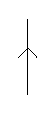
\includegraphics[scale=0.75]{graphics/particleline}
            \caption{Particle line}
        } \qquad
        \parbox{0.35\textwidth}{
            \centering
            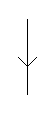
\includegraphics[scale=0.75]{graphics/holeline}
            \caption{Hole line}
        }
    \end{figure}

    \begin{itemize}
        \item Represents a contraction between second quantized operators.
        \item External lines are connected to one operator vertex and infinity.
        \item Internal lines are connected to operator vertices in both ends.
    \end{itemize}

\end{frame}

    

\begin{frame}{Diagram elements - Onebody Hamiltonian}
    \note{Filename: diagram\_hamiltonian01.tex}

    \renewcommand{\figurename}{Level}

    \begin{figure}
    \centering
    \parbox{0.20\textwidth}{
            \centering
            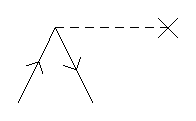
\includegraphics[scale=0.65]{graphics/f1}
            \caption{-1}
        }
        \parbox{0.20\textwidth}{
            \centering
            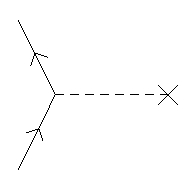
\includegraphics[scale=0.65]{graphics/f2}
            \caption{0}
        }
        \parbox{0.20\textwidth}{
            \centering
            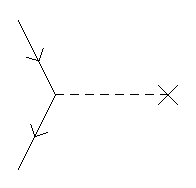
\includegraphics[scale=0.65]{graphics/f3}
            \caption{0}
        }
        \parbox{0.20\textwidth}{
            \centering
            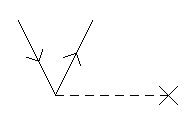
\includegraphics[scale=0.65]{graphics/f4}
            \caption{+1}
        }
    \end{figure}

    \begin{itemize}
        \item Horisontal dashed line segment with one vertex.
        \item Excitation level identify the number of particle/hole pairs created by the operator.
    \end{itemize}
\end{frame}

    

\begin{frame}{Diagram elements - Twobody Hamiltonian}
    \note{Filename: diagram\_hamiltonian02.tex}

    \renewcommand{\figurename}{Level}

    \begin{figure}
    \centering
    \parbox{0.30\textwidth}{
            \centering
            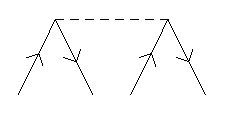
\includegraphics[scale=0.45]{graphics/v1}
            \caption{-2}
        }\quad
        \parbox{0.30\textwidth}{
            \centering
            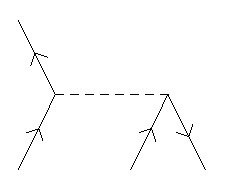
\includegraphics[scale=0.45]{graphics/v2}
            \caption{-1}
        }\quad
        \parbox{0.30\textwidth}{
            \centering
            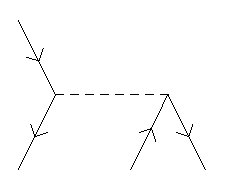
\includegraphics[scale=0.45]{graphics/v3}
            \caption{-1}
        }
    \end{figure}

    \begin{figure}
    \centering
    \parbox{0.30\textwidth}{
            \centering
            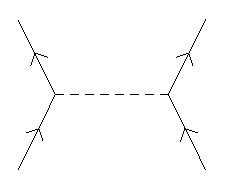
\includegraphics[scale=0.45]{graphics/v4}
            \caption{0}
        }\quad
        \parbox{0.30\textwidth}{
            \centering
            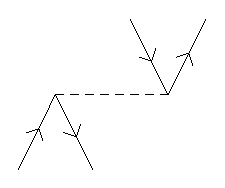
\includegraphics[scale=0.45]{graphics/v5}
            \caption{0}
        }\quad
        \parbox{0.30\textwidth}{
            \centering
            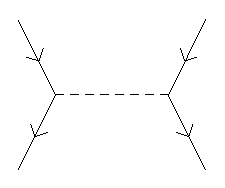
\includegraphics[scale=0.45]{graphics/v6}
            \caption{0}
        }
    \end{figure}

    \begin{figure}
    \centering
    \parbox{0.30\textwidth}{
            \centering
            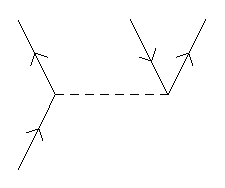
\includegraphics[scale=0.45]{graphics/v7}
            \caption{+1}
        }\quad
        \parbox{0.30\textwidth}{
            \centering
            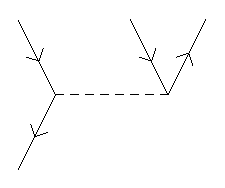
\includegraphics[scale=0.45]{graphics/v8}
            \caption{+1}
        }\quad
        \parbox{0.30\textwidth}{
            \centering
            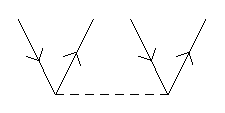
\includegraphics[scale=0.45]{graphics/v9}
            \caption{+2}
        }
    \end{figure}

\end{frame}

    

\begin{frame}{Diagram elements - Onebody cluster operator}
    \note{Filename: diagram\_cc01.tex}

    \renewcommand{\figurename}{Level}

    \begin{figure}
    \centering
    \parbox{0.20\textwidth}{
            \centering
            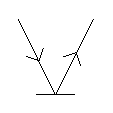
\includegraphics[scale=0.65]{graphics/t1}
            \caption{+1}
        }
    \end{figure}

    \begin{itemize}
        \item Horisontal line segment with one vertex.
        \item Excitation level of +1.
    \end{itemize}
\end{frame}

    

\begin{frame}{Diagram elements - Twobody cluster operator}
    \note{Filename: diagram\_cc02.tex}

    \renewcommand{\figurename}{Level}

    \begin{figure}
    \centering
    \parbox{0.20\textwidth}{
            \centering
            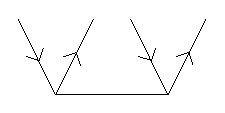
\includegraphics[scale=0.65]{graphics/t2}
            \caption{+2}
        }
    \end{figure}

    \begin{itemize}
        \item Horisontal line segment with two vertices.
        \item Excitation level of +2.
    \end{itemize}
\end{frame}

    

\begin{frame}{CCSD energy equation - Derivation }
    \note{Filename: ccsd\_diagramderivation01.tex}

    \begin{equation*}
        \mathrm{E}_{\mathrm{CCSD}} = \bra{\Phi_0} \barh \ket{\Phi_0}
    \end{equation*}
    \begin{columns}
    \column{0.5\textwidth}
    \begin{itemize}
        \item No external lines.
        \item Final excitation level: 0 
    \end{itemize}
    \column{0.5\textwidth}
    \begin{figure}
        \centering
        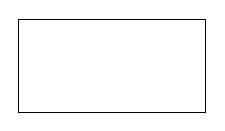
\includegraphics[scale=0.65]{graphics/energy_diag}
    \end{figure}
    \end{columns}
    \renewcommand{\figurename}{Elements}
    \begin{columns}[t]
    \column{0.75\textwidth}
    \begin{figure}
        \caption{$\op{H}_N$}
        \centering
        \parbox{0.20\textwidth}{
            \centering
            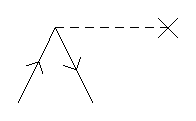
\includegraphics[scale=0.35]{graphics/f1}} 
        \parbox{0.20\textwidth}{
            \centering
            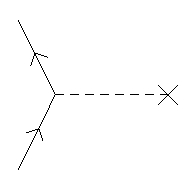
\includegraphics[scale=0.35]{graphics/f2}} 
        \parbox{0.20\textwidth}{
            \centering
            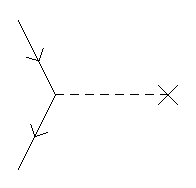
\includegraphics[scale=0.35]{graphics/f3}} 
        \parbox{0.20\textwidth}{
            \centering
            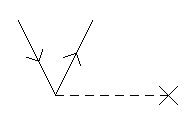
\includegraphics[scale=0.35]{graphics/f4}} 
        \parbox{0.20\textwidth}{
            \centering
            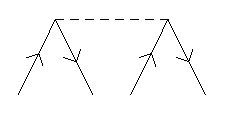
\includegraphics[scale=0.35]{graphics/v1}} 
        \parbox{0.20\textwidth}{
            \centering
            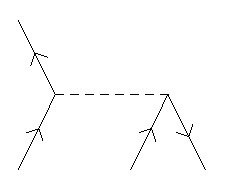
\includegraphics[scale=0.35]{graphics/v2}} 
        \parbox{0.20\textwidth}{
            \centering
            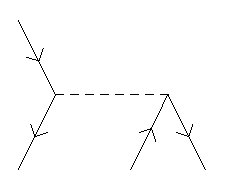
\includegraphics[scale=0.35]{graphics/v3}} 
        \parbox{0.20\textwidth}{
            \centering
            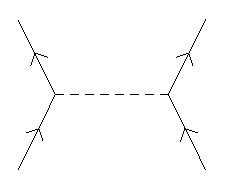
\includegraphics[scale=0.35]{graphics/v4}} 
        \parbox{0.20\textwidth}{
            \centering
            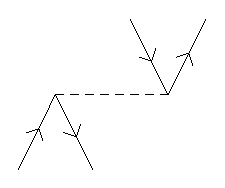
\includegraphics[scale=0.35]{graphics/v5}} 
        \parbox{0.20\textwidth}{
            \centering
            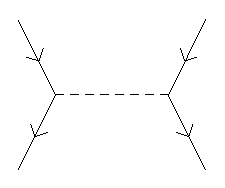
\includegraphics[scale=0.35]{graphics/v6}} 
        \parbox{0.20\textwidth}{
            \centering
            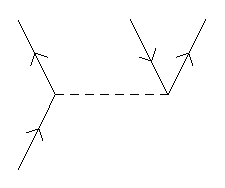
\includegraphics[scale=0.35]{graphics/v7}} 
        \parbox{0.20\textwidth}{
            \centering
            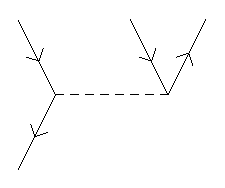
\includegraphics[scale=0.35]{graphics/v8}} 
        \parbox{0.20\textwidth}{
            \centering
            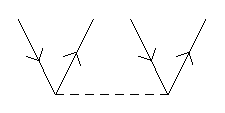
\includegraphics[scale=0.35]{graphics/v9}} 
    \end{figure}
    \column{0.25\textwidth}
    \begin{figure}
        \caption{$\op{T}$}
        \centering
        \parbox[height=3cm]{0.60\textwidth}{
            \centering
            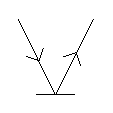
\includegraphics[scale=0.45]{graphics/t1}} 
    \end{figure}
    \begin{figure}
        \parbox[height=3cm]{0.60\textwidth}{
            \centering
            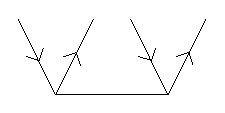
\includegraphics[scale=0.45]{graphics/t2}} 
    \end{figure}
\end{columns}


\end{frame}

    

\begin{frame}{CCSD energy equation }
    \note{Filename: ccsd\_diagramequations01.tex}
    \begin{equation*}
    E_{CCSD} = 
    \parbox{15mm}{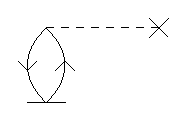
\includegraphics[scale=0.5]{graphics/ccsd_e1}}
    + \parbox{15mm}{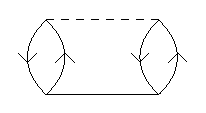
\includegraphics[scale=0.5]{graphics/ccsd_e2}}
    + \parbox{15mm}{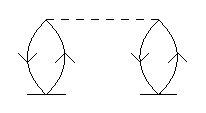
\includegraphics[scale=0.5]{graphics/ccsd_e3}}
\end{equation*}



\end{frame}

    

\begin{frame}{Diagram rules }
    \note<6>{Filename: diagram\_rules01.tex}

    \begin{itemize}
        \item Label all lines. \pause
        \item Sum over all internal indices. \pause
        \item Extract matrix elements. 
            ($f_{\mathrm{in}}^{\mathrm{out}}$, 
            $\bra{\mathrm{lout, rout}}\ket{\mathrm{lin, rin}}$) \pause
        \item Extract cluster amplitudes with indices in the order left to right. Incoming lines are subscripts, while outgoing lines are superscripts. ($t_{\mathrm{in}}^{\mathrm{out}}$,
                        $t^{\mathrm{lout, rout}}_{\mathrm{lin, rin}}$)\pause
        \item Calculate the phase: $(-1)^{\mathrm{holelines} + \mathrm{loops}}$ \pause
        \item Multiply by a factor of $\frac{1}{2}$ for each equivalent line and each ecuivalent vertex.
    \end{itemize}

\end{frame}

    


\begin{frame}{CCSD energy equation }
    \note{Filename: ccsd\_algebraicequations02.tex}
    \begin{equation*}
    E_{CCSD} = 
    f_a^i t_i^a + \frac{1}{4} \bra{ij}\ket{ab} t_{ij}^{ab} + \frac{1}{2} \bra{ij}\ket{ab}  t_i^a  t_j^b
\end{equation*}

Note the implicit sum over repeated indices.



\end{frame}

    



\begin{frame}{CCSD $\op{T}_1$ amplitude equation - Derivation }
    \note{Filename: ccsd\_diagramderivation02.tex}

    \small
    \begin{equation*}
        0 = \bra{\Phi_i^a} \barh \ket{\Phi_0}
    \end{equation*}
    \begin{columns}
    \column{0.5\textwidth}
    \begin{itemize}
        \item One pair of particle/hole  external lines.
        \item Final excitation level: +1
    \end{itemize}
    \column{0.5\textwidth}
    \begin{figure}
        \centering
        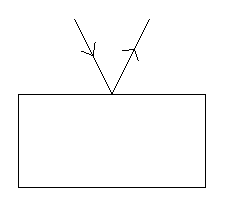
\includegraphics[scale=0.45]{graphics/t1amp_diag}
    \end{figure}
    \end{columns}
    \renewcommand{\figurename}{Elements}
    \begin{columns}[t]
    \column{0.75\textwidth}
    \begin{figure}
        \caption{$\op{H}_N$}
        \centering
        \parbox{0.20\textwidth}{
            \centering
            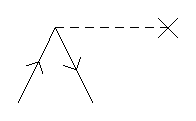
\includegraphics[scale=0.35]{graphics/f1}} 
        \parbox{0.20\textwidth}{
            \centering
            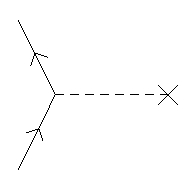
\includegraphics[scale=0.35]{graphics/f2}} 
        \parbox{0.20\textwidth}{
            \centering
            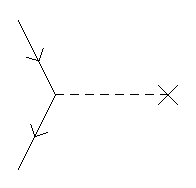
\includegraphics[scale=0.35]{graphics/f3}} 
        \parbox{0.20\textwidth}{
            \centering
            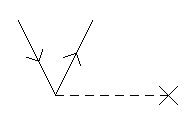
\includegraphics[scale=0.35]{graphics/f4}} 
        \parbox{0.20\textwidth}{
            \centering
            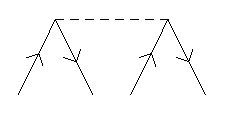
\includegraphics[scale=0.35]{graphics/v1}} 
        \parbox{0.20\textwidth}{
            \centering
            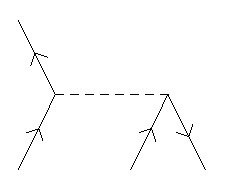
\includegraphics[scale=0.35]{graphics/v2}} 
        \parbox{0.20\textwidth}{
            \centering
            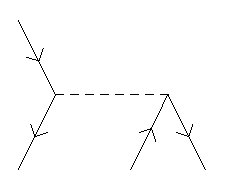
\includegraphics[scale=0.35]{graphics/v3}} 
        \parbox{0.20\textwidth}{
            \centering
            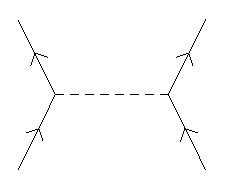
\includegraphics[scale=0.35]{graphics/v4}} 
        \parbox{0.20\textwidth}{
            \centering
            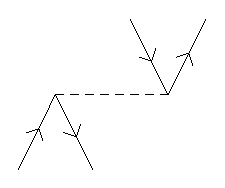
\includegraphics[scale=0.35]{graphics/v5}} 
        \parbox{0.20\textwidth}{
            \centering
            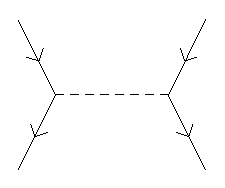
\includegraphics[scale=0.35]{graphics/v6}} 
        \parbox{0.20\textwidth}{
            \centering
            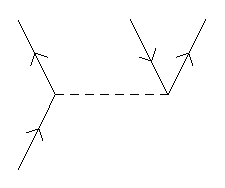
\includegraphics[scale=0.35]{graphics/v7}} 
        \parbox{0.20\textwidth}{
            \centering
            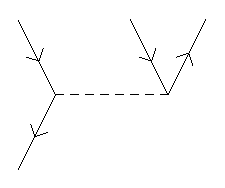
\includegraphics[scale=0.35]{graphics/v8}} 
        \parbox{0.20\textwidth}{
            \centering
            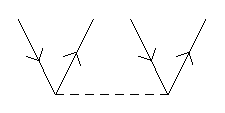
\includegraphics[scale=0.35]{graphics/v9}} 
    \end{figure}
    \column{0.25\textwidth}
    \begin{figure}
        \caption{$\op{T}$}
        \centering
        \parbox[height=3cm]{0.60\textwidth}{
            \centering
            \includegraphics[scale=0.45]{graphics/t1}} 
    \end{figure}
    \begin{figure}
        \parbox[height=3cm]{0.60\textwidth}{
            \centering
            \includegraphics[scale=0.45]{graphics/t2}} 
    \end{figure}
\end{columns}


\end{frame}

    

\begin{frame}{CCSD $\op{T}_1$ amplitude equation }
    \note{Filename: ccsd\_diagramequations02.tex}

\begin{align*}
    0 &= 
    \parbox{10mm}{\includegraphics[scale=0.4]{graphics/ccsd_hbar_04a}}
    + \parbox{18mm}{\includegraphics[scale=0.4]{graphics/ccsd_hbar_04b}}
    + \parbox{15mm}{\includegraphics[scale=0.4]{graphics/ccsd_hbar_04c}}
    + \parbox{15mm}{\includegraphics[scale=0.4]{graphics/ccsd_hbar_04d}} \\
    & \quad + \parbox{21mm}{\includegraphics[scale=0.4]{graphics/ccsd_hbar_04e}}
    + \parbox{17mm}{\includegraphics[scale=0.4]{graphics/ccsd_hbar_04f}}
    + \parbox{15mm}{\includegraphics[scale=0.4]{graphics/ccsd_hbar_04g}}
    + \parbox{15mm}{\includegraphics[scale=0.4]{graphics/ccsd_hbar_04h}} \\
    & \quad + \parbox{17mm}{\includegraphics[scale=0.4]{graphics/ccsd_hbar_04i}}
    + \parbox{15mm}{\includegraphics[scale=0.4]{graphics/ccsd_hbar_04j}}
    + \parbox{20mm}{\includegraphics[scale=0.4]{graphics/ccsd_hbar_04k}}
    + \parbox{15mm}{\includegraphics[scale=0.4]{graphics/ccsd_hbar_04l}} \\
    & \quad + \parbox{17mm}{\includegraphics[scale=0.4]{graphics/ccsd_hbar_04m}}
    + \parbox{15mm}{\includegraphics[scale=0.4]{graphics/ccsd_hbar_04n}}
\end{align*}

\end{frame}

    

\begin{frame}{Diagram rules }
    \note<6>{Filename: diagram\_rules01.tex}

    \begin{itemize}
        \item Label all lines. \pause
        \item Sum over all internal indices. \pause
        \item Extract matrix elements. 
            ($f_{\mathrm{in}}^{\mathrm{out}}$, 
            $\bra{\mathrm{lout, rout}}\ket{\mathrm{lin, rin}}$) \pause
        \item Extract cluster amplitudes with indices in the order left to right. Incoming lines are subscripts, while outgoing lines are superscripts. ($t_{\mathrm{in}}^{\mathrm{out}}$,
                        $t^{\mathrm{lout, rout}}_{\mathrm{lin, rin}}$)\pause
        \item Calculate the phase: $(-1)^{\mathrm{holelines} + \mathrm{loops}}$ \pause
        \item Multiply by a factor of $\frac{1}{2}$ for each equivalent line and each ecuivalent vertex.
    \end{itemize}

\end{frame}

    


\begin{frame}{CCSD $\op{T}_1$ amplitude equation }
    \note{Filename: ccsd\_algebraicequations02.tex}

\begin{align*}
    0 &= f_{i}^a + f_{e}^a t_i^e - f_{i}^mt_m^a + \bra{ma}\ket{ei} t_m^e 
        + f_{e}^m t_{im}^{ae} + \frac{1}{2} \bra{am}\ket{ef} t_{im}^{ef} \\
        &\, - \frac{1}{2} \bra{mn}\ket{ei} t_{mn}^{ea} - f_{e}^m t_i^e t_m^a
        + \bra{am}\ket{ef} t_i^e t_m^f - \bra{mn}\ket{ei} t_m^e t_n^a  \\
        & \quad + \bra{mn}\ket{ef} t_m^e t_{ni}^{fa}
        - \frac{1}{2} \bra{mn}\ket{ef} t_i^e t_{mn}^{af}
        - \frac{1}{2} \bra{mn}\ket{ef} t_n^a t_{mi}^{ef}\\
        & \quad  - \bra{mn}\ket{ef} t_i^e t_m^a t_n^f
\end{align*}


\end{frame}

    


\begin{frame}{CCSD $\op{T}_2$ amplitude equation - Derivation }
    \note{Filename: ccsd\_diagramderivation03.tex}

    \begin{equation*}
        0 = \bra{\Phi_{ij}^{ab}} \barh \ket{\Phi_0}
    \end{equation*}
    \begin{columns}
    \column{0.5\textwidth}
    \begin{itemize}
        \item Two pairs of particle/hole  external lines.
        \item Final excitation level: +2
    \end{itemize}
    \column{0.5\textwidth}
    \begin{figure}
        \centering
        \includegraphics[scale=0.45]{graphics/t2amp_diag}
    \end{figure}
    \end{columns}
    \renewcommand{\figurename}{Elements}
    \begin{columns}[t]
    \column{0.75\textwidth}
    \begin{figure}
        \caption{$\op{H}_N$}
        \centering
        \parbox{0.20\textwidth}{
            \centering
            \includegraphics[scale=0.35]{graphics/f1}} 
        \parbox{0.20\textwidth}{
            \centering
            \includegraphics[scale=0.35]{graphics/f2}} 
        \parbox{0.20\textwidth}{
            \centering
            \includegraphics[scale=0.35]{graphics/f3}} 
        \parbox{0.20\textwidth}{
            \centering
            \includegraphics[scale=0.35]{graphics/f4}} 
        \parbox{0.20\textwidth}{
            \centering
            \includegraphics[scale=0.35]{graphics/v1}} 
        \parbox{0.20\textwidth}{
            \centering
            \includegraphics[scale=0.35]{graphics/v2}} 
        \parbox{0.20\textwidth}{
            \centering
            \includegraphics[scale=0.35]{graphics/v3}} 
        \parbox{0.20\textwidth}{
            \centering
            \includegraphics[scale=0.35]{graphics/v4}} 
        \parbox{0.20\textwidth}{
            \centering
            \includegraphics[scale=0.35]{graphics/v5}} 
        \parbox{0.20\textwidth}{
            \centering
            \includegraphics[scale=0.35]{graphics/v6}} 
        \parbox{0.20\textwidth}{
            \centering
            \includegraphics[scale=0.35]{graphics/v7}} 
        \parbox{0.20\textwidth}{
            \centering
            \includegraphics[scale=0.35]{graphics/v8}} 
        \parbox{0.20\textwidth}{
            \centering
            \includegraphics[scale=0.35]{graphics/v9}} 
    \end{figure}
    \column{0.25\textwidth}
    \begin{figure}
        \caption{$\op{T}$}
        \centering
        \parbox[height=3cm]{0.60\textwidth}{
            \centering
            \includegraphics[scale=0.45]{graphics/t1}} 
    \end{figure}
    \begin{figure}
        \parbox[height=3cm]{0.60\textwidth}{
            \centering
            \includegraphics[scale=0.45]{graphics/t2}} 
    \end{figure}
\end{columns}


\end{frame}

    
\begin{frame}{CCSD $\op{T}_2$ amplitude equation }
    \note{Filename: ccsd\_diagramequations03.tex}

\begin{align*}
    0 &= 
    \parbox{10mm}{\includegraphics[scale=0.25]{graphics/ccsd_hbar_13_01}} + 
    \parbox{10mm}{\includegraphics[scale=0.25]{graphics/ccsd_hbar_13_02}} + 
    \parbox{10mm}{\includegraphics[scale=0.25]{graphics/ccsd_hbar_13_03}} +
    \parbox{14mm}{\includegraphics[scale=0.25]{graphics/ccsd_hbar_13_04}} + 
    \parbox{14mm}{\includegraphics[scale=0.25]{graphics/ccsd_hbar_13_05}} + 
    \parbox{14mm}{\includegraphics[scale=0.25]{graphics/ccsd_hbar_13_06}} \\
    & + \parbox{14mm}{\includegraphics[scale=0.25]{graphics/ccsd_hbar_13_07}} + 
    \parbox{14mm}{\includegraphics[scale=0.25]{graphics/ccsd_hbar_13_08}} + 
    \parbox{14mm}{\includegraphics[scale=0.25]{graphics/ccsd_hbar_13_09}} +
    \parbox{14mm}{\includegraphics[scale=0.25]{graphics/ccsd_hbar_13_10}} + 
    \parbox{14mm}{\includegraphics[scale=0.25]{graphics/ccsd_hbar_13_11}} \\
    & + \parbox{15mm}{\includegraphics[scale=0.25]{graphics/ccsd_hbar_13_12}} +
    \parbox{19mm}{\includegraphics[scale=0.25]{graphics/ccsd_hbar_13_13}} + 
    \parbox{15mm}{\includegraphics[scale=0.25]{graphics/ccsd_hbar_13_14}} +
    \parbox{15mm}{\includegraphics[scale=0.25]{graphics/ccsd_hbar_13_15}} + 
    \parbox{15mm}{\includegraphics[scale=0.25]{graphics/ccsd_hbar_13_16}} \\
    & + \parbox{15mm}{\includegraphics[scale=0.25]{graphics/ccsd_hbar_13_17}} +
    \parbox{17mm}{\includegraphics[scale=0.25]{graphics/ccsd_hbar_13_18}} + 
    \parbox{15mm}{\includegraphics[scale=0.25]{graphics/ccsd_hbar_13_19}} +
    \parbox{15mm}{\includegraphics[scale=0.25]{graphics/ccsd_hbar_13_20}} + 
    \parbox{15mm}{\includegraphics[scale=0.25]{graphics/ccsd_hbar_13_21}} \\
    & + \parbox{15mm}{\includegraphics[scale=0.25]{graphics/ccsd_hbar_13_22}} + 
    \parbox{15mm}{\includegraphics[scale=0.25]{graphics/ccsd_hbar_13_23}} +
    \parbox{15mm}{\includegraphics[scale=0.25]{graphics/ccsd_hbar_13_24}} + 
    \parbox{15mm}{\includegraphics[scale=0.25]{graphics/ccsd_hbar_13_25}} +
    \parbox{15mm}{\includegraphics[scale=0.25]{graphics/ccsd_hbar_13_26}} \\
    & + \parbox{16mm}{\includegraphics[scale=0.25]{graphics/ccsd_hbar_13_27}} +
    \parbox{17mm}{\includegraphics[scale=0.25]{graphics/ccsd_hbar_13_28}} + 
    \parbox{14mm}{\includegraphics[scale=0.25]{graphics/ccsd_hbar_13_29}} +
    \parbox{15mm}{\includegraphics[scale=0.25]{graphics/ccsd_hbar_13_30}} + 
    \parbox{15mm}{\includegraphics[scale=0.25]{graphics/ccsd_hbar_13_31}}
\end{align*}

\end{frame}

    


\begin{frame}{Diagram rules }
    \begin{itemize}
        \item Label all lines. 
        \item Sum over all internal indices. 
        \item Extract matrix elements. 
            ($f_{\mathrm{in}}^{\mathrm{out}}$, 
            $\bra{\mathrm{lout, rout}}\ket{\mathrm{lin, rin}}$) 
        \item Extract cluster amplitudes with indices in the order left to right. Incoming lines are subscripts, while outgoing lines are superscripts. ($t_{\mathrm{in}}^{\mathrm{out}}$,
                        $t^{\mathrm{lout, rout}}_{\mathrm{lin, rin}}$)
        \item Calculate the phase: $(-1)^{\mathrm{holelines} + \mathrm{loops}}$ 
        \item Multiply by a factor of $\frac{1}{2}$ for each equivalent line and each ecuivalent vertex. 
        \item Antisymmetrize a pair of external particle/hole line that does not connect to the same operator.
    \end{itemize}

\end{frame}

    



\begin{frame}{CCSD $\op{T}_2$ amplitude equation }
    \note{Filename: ccsd\_algebraicequations03.tex}
    \scriptsize
\begin{align*}
    0 &= 
        \bra{ab} \ket{ij}
        + P(ij) \bra{ab}\ket{ej} t_i^e
        - P(ab) \bra{am} \ket{ij} t_m^b
        + P(ab) f_{e}^b t_{ij}^{ae}
        - P(ij) f_{i}^m t_{mj}^{ab} \\
        & + \, \frac{1}{2} \bra{ab}\ket{ef} t_{ij}^{ef}
        + \frac{1}{2} \bra{mn}\ket{ij} t_{mn}^{ab}
        + P(ij) P(ab) \bra{mb}\ket{ej} t_{im}^{ae} \\
        & + \, \frac{1}{2} P(ij) \bra{ab}\ket{ef} t_i^e t_j^f
        + \frac{1}{2} P(ab) \bra{mn}\ket{ij} t_m^a t_n^b
        - P(ij) P(ab) \bra{mb}\ket{ej} t_i^e t_m^a \\
        & + \, \frac{1}{4} \bra{mn}\ket{ef} t_{ij}^{ef} t_{mn}^{ab}
        + \frac{1}{2} P(ij) P(ab) \bra{mn}\ket{ef} t_{im}^{ae} t_{nj}^{fb}
        - \frac{1}{2} P(ab) \bra{mn}\ket{ef} t_{ij}^{ae} t_{mn}^{bf} \\
        & - \, \frac{1}{2} P(ij) \bra{mn}\ket{ef} t_{mi}^{ef} t_{nj}^{ab}
        - P(ij) f_{e}^m t_i^e t_{mj}^{ab}
        - P(ab) f_{e}^m t_{ij}^{ae} t_m^b \\
        & + \, P(ij) P(ab) \bra{am}\ket{ef} t_i^e t_{mj}^{fb}
        - \frac{1}{2} P(ab) \bra{am}\ket{ef} t_{ij}^{ef} t_m^b
        + P(ab) \bra{bm}\ket{ef} t_{ij}^{ae} t_m^f \\
        & - \, P(ij) P(ab) \bra{mn} \ket{ej} t_{im}^{ae} t_n^b
        + \frac{1}{2} P(ij) \bra{mn}\ket{ej} t_i^e t_{mn}^{ab}
        -P(ij) \bra{mn}\ket{ei} t_m^e t_{nj}^{ab} \\
        & - \, \frac{1}{2} P(ij) P(ab) \bra{am}\ket{ef} t_i^e t_j^f t_m^b
        + \frac{1}{2} P(ij) P(ab) \bra{mn}\ket{ej} t_i^e t_m^a t_n^b \\
        & + \, \frac{1}{4} P(ij) \bra{mn}\ket{ef} t_i^e t_{mn}^{ab} t_j^f
        - P(ij) P(ab) \bra{mn}\ket{ef} t_i^e t_m^a t_{nj}^{fb} \\
        & + \, \frac{1}{4} P(ab) \bra{mn}\ket{ef} t_m^a t_{ij}^{ef} t_n^b
        - P(ij) \bra{mn}\ket{ef} t_m^e t_i^f t_{nj}^{ab}
        - P(ab) \bra{mn}\ket{ef} t_{ij}^{ae} t_m^b t_n^f \\
        & + \, \frac{1}{4} P(ij) P(ab) \bra{mn}\ket{ef} t_i^e t_m^a t_j^f t_n^b \\
\end{align*}

\end{frame}

    

\begin{frame}{The $\barh$ expansion}
    \note{Filename: ccsd\_barh\_expansion01.tex}
        \small
        \begin{align*}
            E_{CC} &= \bra{\Psi_0}\Bigl( \hat{H}_N + \left[ \hat{H}_N, \hat{T} \right] +
                \frac{1}{2} \left[\left[ \hat{H}_N, \hat{T} \right], \hat{T}\right]
                + \frac{1}{3!} \left[ \left[\left[ \hat{H}_N, \hat{T} \right], \hat{T}\right], \hat{T} \right] \\
                & \quad + \frac{1}{4!} \left[ \left[ \left[\left[ \hat{H}_N, \hat{T} \right], \hat{T}\right], \hat{T} \right], \hat{T} \right] ++ \Bigr) \ket{\Psi_0} \\
        \end{align*}
        \begin{align*}
            0 &= \bra{\Psi_{ij\ldots}^{ab\ldots}}\Bigl( \hat{H}_N + \left[ \hat{H}_N, \hat{T} \right] +
                \frac{1}{2} \left[\left[ \hat{H}_N, \hat{T} \right], \hat{T}\right]
                + \frac{1}{3!} \left[ \left[\left[ \hat{H}_N, \hat{T} \right], \hat{T}\right], \hat{T} \right] \\
                & \quad + \frac{1}{4!} \left[ \left[ \left[\left[ \hat{H}_N, \hat{T} \right], \hat{T}\right], \hat{T} \right], \hat{T} \right] ++\Bigr) \ket{\Psi_0} \\
        \end{align*}

\end{frame}

    

\begin{frame}{The CCSD energy equation revisited}
    \note{Filename: ccsd\_barh\_expansion02.tex}
        The expanded CC energy equation involves an infinite sum over nested commutators
        \begin{align*}
            E_{CC} &= \bra{\Psi_0}\Bigl( \hat{H}_N + \left[ \hat{H}_N, \hat{T} \right] +
                \frac{1}{2} \left[\left[ \hat{H}_N, \hat{T} \right], \hat{T}\right] \\
                & \qquad + \frac{1}{3!} \left[ \left[\left[ \hat{H}_N, \hat{T} \right], \hat{T}\right], \hat{T} \right] \\
                & \qquad + \frac{1}{4!} \left[ \left[ \left[\left[ \hat{H}_N, \hat{T} \right], \hat{T}\right], \hat{T} \right], \hat{T} \right] ++ \Bigr) \ket{\Psi_0}, \\
        \end{align*}
        but fortunately we can show that it truncates naturally, depending on the Hamiltonian.
        
    \begin{block}{}
        The first term is zero by construction.
        \begin{equation*}
            \bra{\Psi_0} \op{H}_N \ket{\Psi_0} = 0
        \end{equation*}       
    \end{block}
\end{frame}

    

\begin{frame}{The CCSD energy equation revisited.}
    \note{Filename: ccsd\_barh\_expansion03.tex}
     The second term can be split up into different pieces
    \small
        \begin{align*}
        \bra{\Psi_0}\left[ \hat{H}_N, \hat{T} \right]\ket{\Psi_0} & = 
            \bra{\Psi_0} \Bigl(\left[ \hat{F}_N, \hat{T}_1 \right] + \left[ \hat{F}_N, \hat{T}_2 \right]
            + \left[ \hat{V}_N, \hat{T}_1 \right] + \left[ \hat{V}_N, \hat{T}_2 \right] \Bigr) \ket{\Psi_0}
    \end{align*}

    \begin{block}{}
    Since we need the explicit expressions for the commutators both in the next term and in the amplitude equations, we calculate them separately.
    \end{block}

\end{frame}

    

\begin{frame}{The $\barh$ expansion - $\left[ \hat{F}_N, \hat{T}_1 \right]$}
    \note{Filename: ccsd\_barh\_expansion04.tex}
    \begin{align*}
        \left[ \hat{F}_N, \hat{T}_1 \right] &= \sum_{pqia} \left(f_q^p \normord{a_p^\dagger a_q} 
            t_i^a \normord{a_a^\dagger a_i} - t_i^a \normord{a_a^\dagger a_i} f_q^p \normord{a_p^\dagger a_q} \right) \\
        &= \sum_{pqia} f_q^p t_i^a \left( \normord{a_p^\dagger a_q} \normord{a_a^\dagger a_i} -
                \normord{a_a^\dagger a_i} \normord{a_p^\dagger a_q} \right)
    \end{align*} \pause
        \begin{align*}
            \left\{a_a^\dagger a_i\right\} \left\{a_p^\dagger a_q \right\} &= \normord{a_a^\dagger a_i a_p^\dagger a_q} \pause
                = \normord{a_p^\dagger a_q a_a^\dagger a_i} \\ \pause
        \normord{a_p^\dagger a_q}\normord{a_a^\dagger a_i} &= \normord{a_p^\dagger a_q a_a^\dagger a_i}  \\ \pause
            & \quad + \normord{
               \contraction{}{a}{{}^\dagger_pa_q a^\dagger_a}{a}
                a^\dagger_p a_q a^\dagger_a a_i} +
            \normord{
                \contraction{a^\dagger_p}{a}{{}_q}{a}
                a^\dagger_p a_q a^\dagger_a a_i} \\ \pause
            & \quad + \normord{
                \contraction[1.5ex]{}{a}{{}^\dagger_pa_q a^\dagger_a}{a}
                \contraction{a^\dagger_p}{a}{{}_q}{a}
                a^\dagger_p a_q a^\dagger_a a_i} \\ \pause
            &=  \normord{a_p^\dagger a_q a_a^\dagger a_i} + \delta_{qa} \normord{a_p^\dagger a_i} + \delta_{pi} \normord{a_q a_a^\dagger}
            + \delta_{qa}\delta_{pi}
        \end{align*}
\end{frame}

    

\begin{frame}{The $\barh$ expansion - $\left[ \hat{F}_N, \hat{T}_1 \right]$}
    \note{Filename: ccsd\_barh\_expansion05.tex}

        Wicks theorem gives us
        \begin{align*}
            \left\{a_p^\dagger a_q \right\}\left\{a_a^\dagger a_i\right\} - \left\{a_a^\dagger a_i\right\} \left\{a_p^\dagger a_q \right\} &= \delta_{qa} \left\{ a_p^\dagger a_i\right\} + \delta_{pi} \left\{ a_q a_a^\dagger \right\} + \delta_{qa}\delta_{pi}.
    \end{align*}

        Inserted into the original expression, we arrive at the explicit value of the commutator
        \begin{align*}
        \left[ \hat{F}_N, \hat{T}_1 \right] &= \sum_{pai} f_a^p t_i^a \normord{a_p^\dagger a_i} + 
                \sum_{qai} f_q^i t_i^a \normord{a_q a_a^\dagger} + \sum_{ai} f_a^i t_i^a \\
            &= \left( \op{F}_N \op{T}_1 \right)_c.
        \end{align*}
    The subscript means that the product only includes terms where the operators are connected by atleast one shared index.

\end{frame}

    

\begin{frame}{The $\barh$ expansion - $\left[ \hat{F}_N, \hat{T}_2 \right]$}
    \note{Filename: ccsd\_barh\_expansion06.tex}
    \begin{align*}
        \left[ \hat{F}_N, \hat{T}_2 \right] 
        &= \left[\sum_{pq} f_q^p \normord{a^\dagger_p a_q},
            \frac{1}{4}\sum_{ijab} t_{ij}^{ab} \normord{a^\dagger_a a^\dagger_b a_j a_i} \right] \\
        &= \frac{1}{4}\sum_{\substack{pq\\ijab}}
        \left[ \normord{a^\dagger_p a_q}, \normord{a^\dagger_a a^\dagger_b a_j a_i} \right] \\
        &= \frac{1}{4}\sum_{\substack{pq\\ijab}}
            f_q^p t_{ij}^{ab}
        \left( \normord{a^\dagger_p a_q} \normord{a^\dagger_a a^\dagger_b a_j a_i}
            - \normord{a^\dagger_a a^\dagger_b a_j a_i} \normord{a^\dagger_p a_q} \right)
    \end{align*}
\end{frame}

    

\begin{frame}{The $\barh$ expansion - $\left[ \hat{F}_N, \hat{T}_2 \right]$}
    \note{Filename: ccsd\_barh\_expansion07.tex}
    \small
    \begin{align*}
        \normord{a^\dagger_a a^\dagger_b a_j a_i} \normord{a^\dagger_p a_q} &= 
            \normord{a^\dagger_a a^\dagger_b a_j a_i a^\dagger_p a_q} \\ \pause
        &= \normord{a^\dagger_p a_q a^\dagger_a a^\dagger_b a_j a_i} \pause
        \\
        \normord{a^\dagger_p a_q} \normord{a^\dagger_a a^\dagger_b a_j a_i} &= 
            \normord{a^\dagger_p a_q a^\dagger_a a^\dagger_b a_j a_i} \pause
        + \left\{ 
        \contraction{}{a}{{}^\dagger_pa_q a^\dagger_a a^\dagger_b}{a}
        a^\dagger_p a_q a^\dagger_a a^\dagger_b a_j a_i\right\}
        + \left\{ 
        \contraction{}{a}{{}^\dagger_pa_q a^\dagger_a a^\dagger_b a_j}{a}
        a^\dagger_p a_q a^\dagger_a a^\dagger_b a_j a_i\right\} \\
        & \quad 
        + \left\{ 
        \contraction{a^\dagger_p}{a}{{}_q}{a}
        a^\dagger_p a_q a^\dagger_a a^\dagger_b a_j a_i\right\}
        + \left\{ 
        \contraction{a^\dagger_p}{a}{{}_q a^\dagger_a}{a}
        a^\dagger_p a_q a^\dagger_a a^\dagger_b a_j a_i\right\} \pause
        + \left\{ 
        \contraction{a^\dagger_p}{a}{{}_q}{a}
        \contraction[1.5ex]{}{a}{{}^\dagger_pa_q a^\dagger_a a^\dagger_b}{a}
        a^\dagger_p a_q a^\dagger_a a^\dagger_b a_j a_i\right\} \\
        & \quad 
        + \left\{ 
        \contraction{a^\dagger_p}{a}{{}_q}{a}
        \contraction[1.5ex]{}{a}{{}^\dagger_pa_q a^\dagger_a a^\dagger_b a_j}{a}
        a^\dagger_p a_q a^\dagger_a a^\dagger_b a_j a_i\right\}
        + \left\{ 
        \contraction{a^\dagger_p}{a}{{}_q a^\dagger_a}{a}
        \contraction[1.5ex]{}{a}{{}^\dagger_pa_q a^\dagger_a a^\dagger_b}{a}
        a^\dagger_p a_q a^\dagger_a a^\dagger_b a_j a_i\right\}
        + \left\{ 
        \contraction{a^\dagger_p}{a}{{}_q a^\dagger_a}{a}
        \contraction[1.5ex]{}{a}{{}^\dagger_pa_q a^\dagger_a a^\dagger_b a_j}{a}
        a^\dagger_p a_q a^\dagger_a a^\dagger_b a_j a_i\right\} \\ \pause
        &= \normord{a^\dagger_p a_q a^\dagger_a a^\dagger_b a_j a_i}
        - \delta_{pj} \normord{a_q a^\dagger_a a^\dagger_b a_i}
        + \delta_{pi} \normord{a_q a^\dagger_a a^\dagger_b a_j} \\
        & \quad + \delta_{qa} \normord{a^\dagger_p a^\dagger_b a_j a_i}
        - \delta_{qb}\normord{a^\dagger_p a^\dagger_a a_j a_i} 
        - \delta_{pj} \delta_{qa} \normord{a^\dagger_b a_i} \\
        & \quad + \delta_{pi} \delta_{qa} \normord{a^\dagger_b a_j}
        + \delta_{pj} \delta_{qb} \normord{a^\dagger_a a_i}
        - \delta_{pi} \delta_{qb} \normord{a^\dagger_a a_j}
    \end{align*}

\end{frame}

    

\begin{frame}{The $\barh$ expansion - $\left[ \hat{F}_N, \hat{T}_2 \right]$}
    \note{Filename: ccsd\_barh\_expansion08.tex}
    Wicks theorem gives us
    \small
    \begin{align*}
        & \Bigl( \normord{a^\dagger_p a_q} \normord{a^\dagger_a a^\dagger_b a_j a_i}
            - \normord{a^\dagger_a a^\dagger_b a_j a_i} \normord{a^\dagger_p a_q} \Bigr) = \\
        & \qquad - \delta_{pj} \normord{a_q a^\dagger_a a^\dagger_b a_i}
        + \delta_{pi} \normord{a_q a^\dagger_a a^\dagger_b a_j}
        + \delta_{qa} \normord{a^\dagger_p a^\dagger_b a_j a_i} \\
        & \qquad - \delta_{qb}\normord{a^\dagger_p a^\dagger_a a_j a_i} 
        - \delta_{pj} \delta_{qa} \normord{a^\dagger_b a_i}
        + \delta_{pi} \delta_{qa} \normord{a^\dagger_b a_j}
        + \delta_{pj} \delta_{qb} \normord{a^\dagger_a a_i} \\
        & \qquad - \delta_{pi} \delta_{qb} \normord{a^\dagger_a a_j}
    \end{align*}
    \pause
    Inserted into the original expression, we arrive at
    \begin{align*}
        \left[ \op{F}_N, \op{T}_2 \right]
        &= \frac{1}{4} \sum_{\substack{pq\\abij}} f_q^p t_{ij}^{ab} \Bigl(
        - \delta_{pj} \normord{a_q a^\dagger_a a^\dagger_b a_i}
        + \delta_{pi} \normord{a_q a^\dagger_a a^\dagger_b a_j} \\
        & \quad + \delta_{qa} \normord{a^\dagger_p a^\dagger_b a_j a_i}
        - \delta_{qb}\normord{a^\dagger_p a^\dagger_a a_j a_i} 
        - \delta_{pj} \delta_{qa} \normord{a^\dagger_b a_i} \\
        & \quad + \delta_{pi} \delta_{qa} \normord{a^\dagger_b a_j}
        + \delta_{pj} \delta_{qb} \normord{a^\dagger_a a_i}
        - \delta_{pi} \delta_{qb} \normord{a^\dagger_a a_j} \Bigr).
    \end{align*}

\end{frame}

    

\begin{frame}{The $\barh$ expansion - $\left[ \hat{F}_N, \hat{T}_2 \right]$}
    \note{Filename: ccsd\_barh\_expansion09.tex}

    After renaming indices and changing the order of operators, we arrive at the explicit expression
    \begin{align*}
        \left[ \op{F}_N, \op{T}_2 \right]
        &= \frac{1}{2} \sum_{qijab} f_q^i t_{ij}^{ab} \normord{a_q a^\dagger_a a^\dagger_b a_j}
        + \frac{1}{2} \sum_{pijab} f_a^p t_{ij}^{ab} \normord{a^\dagger_p a^\dagger_b a_j a_i} \\
        & \quad + \sum_{ijab} f_a^i t_{ij}^{ab} \normord{a^\dagger_b a_j} \\
    &= \left( \op{F}_N \op{T}_2\right)_c.
    \end{align*}
    The subscript implies that only the connected terms from the product contribute.

\end{frame}

    

\begin{frame}{The $\barh$ expansion - $\frac{1}{2}\left[ \left[ \op{F}_N, \op{T}_1 \right], \op{T}_1 \right]$}
    \note{Filename: ccsd\_barh\_expansion10.tex}
    \small
        \begin{align*}
        \left[ \hat{F}_N, \hat{T}_1 \right] &= \sum_{pai} f_a^p t_i^a \normord{a_p^\dagger a_i} + 
                \sum_{qai} f_q^i t_i^a \normord{a_q a_a^\dagger} + \sum_{ai} f_a^i t_i^a
        \end{align*}

        \pause
    \begin{align*}
        \left[ \left[ \op{F}_N, \op{T}_1 \right], \op{T}_1\right] 
        &= \Bigl[ \sum_{pai} f_a^p t_i^a \normord{a_p^\dagger a_i} +
            \sum_{qai} f_q^i t_i^a \normord{a_q a_a^\dagger} + \sum_{ai} f_a^i t_i^a, \sum_{jb} t_j^b \normord{a_b^\dagger a_j} \\
        &= \Bigl[ \sum_{pai} f_a^p t_i^a \normord{a_p^\dagger a_i} +
            \sum_{qai} f_q^i t_i^a \normord{a_q a_a^\dagger}, \sum_{jb} t_j^b \normord{a_b^\dagger a_j} \\
        &= \sum_{pabij} f_a^p t_i^a t_j^b \left[ \normord{a_p^\dagger a_i}, \normord{a_b^\dagger a_j} \right] +
            \sum_{qabij} f_q^i t_i^a t_j^b \left[ \normord{a_q a_a^\dagger}, \normord{a_b^\dagger a_j} \right]
    \end{align*}
        \pause
    \begin{align*}
        \normord{a_b^\dagger a_j} \normord{a_p^\dagger a_i} &= \normord{a_b^\dagger a_j a_p^\dagger a_i} 
            = \normord{ a_p^\dagger a_i a_b^\dagger a_j} \\
        \pause
        \normord{a_b^\dagger a_j} \normord{a_q a_a^\dagger} &= \normord{ a_b^\dagger a_j a_q a_a^\dagger} 
            =  \normord{ a_q a_a^\dagger a_b^\dagger a_j}
    \end{align*}
\end{frame}

    

\begin{frame}{The $\barh$ expansion - $\left[ \left[ \op{F}_N, \op{T}_1 \right], \op{T}_1 \right]$}
    \note{Filename: ccsd\_barh\_expansion11.tex}

    \small
    \begin{align*}
        \frac{1}{2} \left[ \left[ \op{F}_N, \op{T}_1 \right], \op{T}_1\right] 
        &= \frac{1}{2} \left(\sum_{pabij} f_a^p t_i^a t_j^b \delta_{pj} \normord{a_i a_b^\dagger}
            - \sum_{qabij} f_q^i t_i^a t_j^b \delta_{qb} \normord{a_a^\dagger a_j}\right) \\
        &= -\frac{1}{2} 2 \sum_{abij} f_b^j t_j^a t_i^b \normord{a_a^\dagger a_i} \\
        &= -\sum_{abij} f_b^j t_j^a t_i^b \normord{a_a^\dagger a_i} \\
        &= \frac{1}{2} \left(  \op{F}_N \op{T}_1^2 \right)_c
    \end{align*}

\end{frame}

    

\begin{frame}{The CCSD energy equation revisited }
    \note{Filename: ccsd\_barh\_expansion12.tex}

    \small
    \begin{align*}
        \bra{\Phi_0} \left[ \hat{V}_N, \hat{T}_1 \right] \ket{\Phi_0} &= 
            \bra{\Phi_0}
                \left[ \frac{1}{4} \sum_{pqrs} \bra{pq}\ket{rs} \normord{a^\dagger_p a^\dagger_q a_s  a_r},
                    \sum_{ia} t_i^a \normord{a^\dagger_a a_i} \right] \ket{\Phi_0} \\ \pause
            &= \frac{1}{4}\sum_{\substack{
                pqr \\
                sia}} \bra{pq}\ket{rs} t_i^a \bra{\Phi_0} 
                \left[ \normord{a^\dagger_p a^\dagger_q a_s  a_r}, \normord{a^\dagger_a a_i} \right]
                \ket{\Phi_0} \\ \pause
        &= 0
    \end{align*}



\end{frame}

    

\begin{frame}{The CCSD energy equation revisited }
    \note{Filename: ccsd\_barh\_expansion13.tex}

    \small
    \begin{align*}
        & \bra{\Phi_0} \left[ \hat{V}_N, \hat{T}_2 \right] \ket{\Phi_0}= \\
            & \quad \bra{\Phi_0}
                \left[ \frac{1}{4} \sum_{pqrs} \bra{pq}\ket{rs} \normord{a^\dagger_p a^\dagger_q a_s  a_r},
                    \frac{1}{4}\sum_{ijab} t_{ij}^{ab} \normord{a^\dagger_a a^\dagger_b a_j a_i} \right] \ket{\Phi_0} \\ \pause
            &= \frac{1}{16}\sum_{\substack{
                    pqr \\
                    sijab}} \bra{pq}\ket{rs}t_{ij}^{ab} \bra{\Phi_0} 
                \left[ \normord{a^\dagger_p a^\dagger_q a_s  a_r}, \normord{a^\dagger_a a^\dagger_b a_j a_i} \right]
                \ket{\Phi_0} \\ \pause
            &= \frac{1}{16}\sum_{\substack{
                    pqr \\
                    sijab}} \bra{pq}\ket{rs}t_{ij}^{ab} \bra{\Phi_0}
            \Bigl(
            \left\{
            \contraction{a^\dagger_p a^\dagger_q a_s}{a}{{}_r}{a}
            \contraction[1.25ex]{a^\dagger_p a^\dagger_q}{a}{{}_s a_r a^\dagger_a}{a}
            \contraction[1.50ex]{a^\dagger_p}{a}{{}^\dagger_q a_s a_r a^\dagger_a a^\dagger_b}{a}
            \contraction[1.75ex]{}{a}{{}^\dagger_p a^\dagger_q a_s a_r a^\dagger_a a^\dagger_b a_j}{a}
            a^\dagger_p a^\dagger_q a_s  a_r a^\dagger_a a^\dagger_b a_j a_i \right\}
            + \left\{
            \contraction{a^\dagger_p a^\dagger_q}{a}{{}_s a_r}{a}
            \contraction[1.25ex]{a^\dagger_p a^\dagger_q a_s}{a}{{}_r a^\dagger_p}{a}
            \contraction[1.50ex]{a^\dagger_p}{a}{{}^\dagger_q a_s a_r a^\dagger_a a^\dagger_b}{a}
            \contraction[1.75ex]{}{a}{{}^\dagger_p a^\dagger_q a_s a_r a^\dagger_a a^\dagger_b a_j}{a}
            a^\dagger_p a^\dagger_q a_s  a_r a^\dagger_a a^\dagger_b a_j a_i \right\} \\
            & \quad \left\{
            \contraction{a^\dagger_p a^\dagger_q a_s}{a}{{}_r}{a}
            \contraction[1.25ex]{a^\dagger_p a^\dagger_q}{a}{{}_s a_r a^\dagger_a}{a}
            \contraction[1.5ex]{}{a}{{}^\dagger_p a^\dagger_q a_s a_r a^\dagger_a a^\dagger_b}{a}
            \contraction[1.75ex]{a^\dagger_p}{a}{{}^\dagger_q a_s a_r a^\dagger_a a^\dagger_b a_j}{a}
            a^\dagger_p a^\dagger_q a_s  a_r a^\dagger_a a^\dagger_b a_j a_i \right\}
            + \left\{
            \contraction{a^\dagger_p a^\dagger_q}{a}{{}_s a_r}{a}
            \contraction[1.25ex]{a^\dagger_p a^\dagger_q a_s}{a}{{}_r a^\dagger_p}{a}
            \contraction[1.5ex]{}{a}{{}^\dagger_p a^\dagger_q a_s a_r a^\dagger_a a^\dagger_b}{a}
            \contraction[1.75ex]{a^\dagger_p}{a}{{}^\dagger_q a_s a_r a^\dagger_a a^\dagger_b a_j}{a}
            a^\dagger_p a^\dagger_q a_s  a_r a^\dagger_a a^\dagger_b a_j a_i \right\}
            \Bigr) \ket{\Phi_0} \\ \pause
            &= \frac{1}{4} \sum_{ijab} \bra{ij}\ket{ab} t_{ij}^{ab}
    \end{align*}


\end{frame}

    

\begin{frame}{The CCSD energy equation revisited }
    \note{Filename: ccsd\_barh\_expansion14.tex}

    The CCSD energy get two contributions from $\left(\op{H}_N \op{T}\right)_c$
    \begin{align*}
        E_{CC} & \Leftarrow \bra{\Phi_0} \left[ \hat{H}_N, \hat{T} \right] \ket{\Phi_0} \\
            &= \sum_{ia} f_a^i t_i^a + \frac{1}{4} \sum_{ijab} \bra{ij}\ket{ab} t_{ij}^{ab}
    \end{align*}



\end{frame}

    

\begin{frame}{The CCSD energy equation revisited }
    \note{Filename: ccsd\_barh\_expansion15.tex}

    \begin{align*}
        E_{CC} & \Leftarrow \bra{\Phi_0} \frac{1}{2} \left( \op{H}_N \op{T}^2 \right)_c \ket{\Phi_0}
     \end{align*}
    \pause
    \small
    \begin{align*}
        & \bra{\Phi_0} \frac{1}{2} \left( \op{V}_N \op{T}_1^2 \right)_c \ket{\Phi_0} = \\
            & \quad \frac{1}{8} \sum_{pqrs} \sum_{ijab} \bra{pq}\ket{rs} t_i^a t_j^b 
            \bra{\Phi_0} \left(\normord{a^\dagger_p a^\dagger_q a_s  a_r} 
            \normord{a^\dagger_a a_i} \normord{a^\dagger_b a_j} \right)_c\ket{\Phi_0} \\ \pause
        &= \frac{1}{8} \sum_{pqrs} \sum_{ijab} \bra{pq}\ket{rs} t_i^a t_j^b \bra{\Phi_0} \\
        & \quad \Bigl( 
        \left\{
        \contraction{a^\dagger_p a^\dagger_q a_s}{a}{{}_r}{a}
        \contraction[1.25ex]{a^\dagger_p}{a}{{}^\dagger_q a_s a_r a^\dagger_a}{a}
        \contraction[1.5ex]{a^\dagger_p a^\dagger_q }{a}{{}_s a_r a^\dagger_a a_i}{a}
        \contraction[1.75ex]{}{a}{{}^\dagger_p a^\dagger_q a_s a_r a^\dagger_a a_i a^\dagger_b}{a}
        a^\dagger_p a^\dagger_q a_s  a_r a^\dagger_a a_i a^\dagger_b a_j \right\}
        +\left\{
        \contraction{a^\dagger_p a^\dagger_q}{a}{{}_s a_r}{a}
        \contraction[1.25ex]{a^\dagger_p}{a}{{}^\dagger_q a_s a_r a^\dagger_a}{a}
        \contraction[1.5ex]{a^\dagger_p a^\dagger_q a_s}{a}{{}_r a^\dagger_a a_i}{a}
        \contraction[1.75ex]{}{a}{{}^\dagger_p a^\dagger_q a_s a_r a^\dagger_a a_i a^\dagger_b}{a}
        a^\dagger_p a^\dagger_q a_s  a_r a^\dagger_a a_i a^\dagger_b a_j \right\}
        + \left\{
        \contraction{a^\dagger_p a^\dagger_q a_s}{a}{{}_r}{a}
        \contraction[1.25ex]{}{a}{{}^\dagger_p q^\dagger_q a_s a_r a^\dagger_a}{a}
        \contraction[1.5ex]{a^\dagger_p a^\dagger_q }{a}{{}_s a_r a^\dagger_a a_i}{a}
        \contraction[1.75ex]{a^\dagger_p}{a}{{}^\dagger_q a_s a_r a^\dagger_a a_i a^\dagger_b}{a}
        a^\dagger_p a^\dagger_q a_s  a_r a^\dagger_a a_i a^\dagger_b a_j \right\} \\
        & \quad +\left\{
        \contraction{a^\dagger_p a^\dagger_q}{a}{{}_s a_r}{a}
        \contraction[1.25ex]{}{a}{{}^\dagger_p q^\dagger_q a_s a_r a^\dagger_a}{a}
        \contraction[1.5ex]{a^\dagger_p a^\dagger_q a_s}{a}{{}_r a^\dagger_a a_i}{a}
        \contraction[1.75ex]{a^\dagger_p}{a}{{}^\dagger_q a_s a_r a^\dagger_a a_i a^\dagger_b}{a}
        a^\dagger_p a^\dagger_q a_s  a_r a^\dagger_a a_i a^\dagger_b a_j \right\}
        \Bigr) \ket{\Phi_0} \\ \pause
        &= \frac{1}{2} \sum_{ijab} \bra{ij}\ket{ab} t_i^a t_j^b
    \end{align*}



\end{frame}

    

\begin{frame}{The CCSD energy equation revisited }
    \note{Filename: ccsd\_barh\_expansion16.tex}

    \begin{itemize}
        \item No contractions possible between cluster operators. \pause
        \item Cluster operators need to contract with free indices to the left. \pause
        \item Disconnected parts automatically cancel in the commutator. \pause
        \item Onebody operators can connect to maximum two cluster operators. \pause
        \item Twobody operators can connect to maximum four cluster operators. \pause
        \item Different terms in the $\barh$ expansion contributes to different equations.
    \end{itemize}


\end{frame}

    


\begin{frame}
    \frametitle{Factoring, motivation}
\note{Filename: ccsd\_factoring01.tex}

\small
\begin{block}{Diagram (2.12)}
    \begin{equation*}
        \parbox{40mm}{\includegraphics[scale=0.5]{graphics/ccsd_hbar_13_12}}
        = \frac{1}{4}  \bra{mn}\ket{ef} t_{ij}^{ef} t_{mn}^{ab}
    \end{equation*}
\end{block}
\begin{block}{Diagram (2.26)}
    \begin{equation*}
        \parbox{40mm}{\includegraphics[scale=0.5]{graphics/ccsd_hbar_13_26}}
        = \frac{1}{4} P(ij) \bra{mn}\ket{ef} t_i^e t_{mn}^{ab} t_j^f
    \end{equation*}
\end{block}
\begin{block}{Diagram (2.31)}
    \begin{equation*}
        \parbox{40mm}{\includegraphics[scale=0.5]{graphics/ccsd_hbar_13_31}}
        = \frac{1}{4} P(ij) P(ab) \bra{mn}\ket{ef} t_i^e t_m^a t_j^f t_n^b
    \end{equation*}
\end{block}
\end{frame}


\begin{frame}
    \frametitle{Factoring, motivation}
\note{Filename: ccsd\_factoring02.tex}

\scriptsize
\begin{block}{Diagram (2.12)}
    \begin{equation*}
        \parbox{40mm}{\includegraphics[scale=0.5]{graphics/ccsd_hbar_13_12}}
        = \frac{1}{4}  \bra{mn}\ket{ef} t_{ij}^{ef} t_{mn}^{ab}
    \end{equation*}
\end{block}
Diagram cost: $n_p^4 n_h^4$
\begin{block}{Diagram (2.13) - Factored}
\small
    \begin{align*}
        \parbox{40mm}{\includegraphics[scale=0.5]{graphics/ccsd_hbar_13_12}}
        &= \frac{1}{4}  \bra{mn}\ket{ef} t_{ij}^{ef} t_{mn}^{ab} \nn
        &= \frac{1}{4}  \left(\bra{mn}\ket{ef} t_{ij}^{ef}\right)  t_{mn}^{ab} \nn
        &= \frac{1}{4} X_{ij}^{mn} t_{mn}^{ab}
    \end{align*}
\end{block}
\end{frame}


\begin{frame}
    \frametitle{Factoring, motivation}
\note{Filename: ccsd\_factoring03.tex}

\small
\begin{block}{Diagram (2.26)}
    \begin{align*}
        \parbox{40mm}{\includegraphics[scale=0.5]{graphics/ccsd_hbar_13_26}}
        &= \frac{1}{4} P(ij) \bra{mn}\ket{ef} t_i^e t_{mn}^{ab} t_j^f
    \end{align*}
\end{block}
Diagram cost: $n_p^4 n_h^4$
\begin{block}{Diagram (2.26) - Factored}
    \begin{align*}
        \parbox{40mm}{\includegraphics[scale=0.5]{graphics/ccsd_hbar_13_26}}
        &= \frac{1}{4} P(ij) \bra{mn}\ket{ef} t_i^e t_{mn}^{ab} t_j^f \nn
        &= \frac{1}{4} P(ij) t_{mn}^{ab} t_i^e X_{ej}^{mn} \nn
        &= \frac{1}{4} P(ij) t_{mn}^{ab} Y^{mn}_{ij}
    \end{align*}
\end{block}
\end{frame}



\begin{frame}
    \frametitle{Factoring, motivation}
\note{Filename: ccsd\_factoring04.tex}

\scriptsize
\begin{block}{Diagram (2.31)}
    \begin{align*}
        \parbox{40mm}{\includegraphics[scale=0.5]{graphics/ccsd_hbar_13_31}}
        &= \frac{1}{4} P(ij) P(ab) \bra{mn}\ket{ef} t_i^e t_m^a t_j^f t_n^b
    \end{align*}
\end{block}
Diagram cost: $n_p^4 n_h^4$
\begin{block}{Diagram (2.31) - Factored}
    \begin{align*}
        \parbox{40mm}{\includegraphics[scale=0.4]{graphics/ccsd_hbar_13_31}}
        &= \frac{1}{4} P(ij) P(ab) \bra{mn}\ket{ef} t_i^e t_m^a t_j^f t_n^b \nn
        &= \frac{1}{4} P(ij) P(ab) t_m^a t_n^b t_i^e X_{ej}^{mn} \nn
        &= \frac{1}{4} P(ij) P(ab) t_m^a t_n^b Y_{ij}^{mn} \nn
        &= \frac{1}{4} P(ij) P(ab) t_m^a Z_{ij}^{mb}
    \end{align*}
\end{block}
\end{frame}

\begin{frame}
    \frametitle{Factoring, Classification}
\note{Filename: ccsd\_factoring05.tex}

A diagram is classified by how many hole and particle lines between a $\hat{T}_i$ operator and the interaction ($T_i(p^{np} h^{nh})$).
\begin{block}{Diagram (2.12) Classification}
    \begin{equation*}
        \parbox{40mm}{\includegraphics[scale=0.5]{graphics/ccsd_hbar_13_12}}
        = \frac{1}{4}  \bra{mn}\ket{ef} t_{ij}^{ef} t_{mn}^{ab}
    \end{equation*}
\end{block}
This diagram is classified as $T_2(p^2) \times T_2(h^2)$
\end{frame}



\begin{frame}
    \frametitle{Factoring, Classification}
\note{Filename: ccsd\_factoring06.tex}

\begin{block}{Diagram (2.26)} 
    \begin{equation*}
        \parbox{40mm}{\includegraphics[scale=0.5]{graphics/ccsd_hbar_13_26}}
        = \frac{1}{4} P(ij) \bra{mn}\ket{ef} t_i^e t_{mn}^{ab} t_j^f
    \end{equation*}
\end{block}
This diagram is classified as $T_2(h^2) \times T_1(p) \times T_1(p)$
\begin{block}{Diagram (2.31)} 
    \begin{equation*}
        \parbox{40mm}{\includegraphics[scale=0.5]{graphics/ccsd_hbar_13_31}}
        = \frac{1}{4} P(ij) P(ab) \bra{mn}\ket{ef} t_i^e t_m^a t_j^f t_n^b
    \end{equation*}
\end{block}
This diagram is classified as $T_1(p) \times T_1(p) \times T_1(h) \times T_1(h)$
\end{frame}


\begin{frame}
    \frametitle{Factoring, Classification}
\note{Filename: ccsd\_factoring07.tex}

\begin{block}{\centering Cost of making intermediates}
\begin{center}
\begin{tabular}{|l||c|c|}
    \hline
    Object & CPU cost & Memory cost \\
    \hline
    $T_2(h)$ & $n_p^2 n_h$ & $ n_p^2$ \\
    \hline
    $T_2(h^2)$ & $n_p^2$ & $ n_h^{-2} n_p^2$ \\
    \hline
    $T_2(p)$ & $n_p n_h^2$ & $ n_h^2$ \\
    \hline
    $T_2(ph)$ & $n_p n_h$ & $1$ \\
    \hline
    $T_1(h)$ & $n_p$ & $ n_h^{-1} n_p$ \\
    \hline
    $T_2(ph^2)$ & $n_p$ & $ n_h^{-2}$ \\
    \hline
    $T_2(p^2)$ & $ n_h^2$ & $ n_p^{-2} n_h^2$ \\
    \hline
    $T_1(p)$ & $n_h$ & $ n_p^{-1} n_h$ \\
    \hline
    $T_2(p^2h)$ & $n_h$ & $ n_p^{-2}$ \\
    \hline
    $T_1(ph)$ & $1$ & $ n_p^{-1} n_h^{-1}$ \\
    \hline
\end{tabular}
\end{center}

\end{block}
\end{frame}


\begin{frame}
    \frametitle{Factoring, Classification}
\note{Filename: ccsd\_factoring11.tex}

\begin{block}{Classification of $\hat{T}_1$ diagrams}
\begin{tabular}{|l||l|}
    \hline
    Object & Expression id \\
    \hline
    $T_2(ph)$ & 5, 11\\
    \hline
    $T_1(h)$ & 3, 8, 10, 13, 14\\
    \hline
    $T_2(ph^2)$ & 7, 12\\
    \hline
    $T_1(p)$ & 2, 8, 9, 12, 14 \\
    \hline
    $T_2(p^2h)$ & 6, 13\\
    \hline
    $T_1(ph)$ & 4, 9, 10, 11, 14\\
    \hline
\end{tabular}

\end{block}
\end{frame}



\begin{frame}
    \frametitle{Factoring, Classification}
\note{Filename: ccsd\_factoring08.tex}

\begin{block}{Classification of $\hat{T}_2$ diagrams}
\small
\begin{tabular}{|l||l|}
    \hline
    Object & Expression id \\
    \hline
    $T_2(h)$ & 5, 15, 16, 23, 29 \\
    \hline
    $T_2(h^2)$ & 7, 12, 22, 26 \\
    \hline
    $T_2(p)$ & 4, 14, 17, 20, 30 \\
    \hline
    $T_2(ph)$ & 8, 13, 13, 18, 21, 27 \\
    \hline
    $T_1(h)$ & 3, 10, 10, 11, 17, 19, 21, 24, 25, 25, 27, 28, 28, 30, 31, 31 \\
    \hline
    $T_2(ph^2)$ & 14 \\
    \hline
    $T_2(p^2)$ & 6, 12, 19, 28 \\
    \hline
    $T_1(p)$ & 2, 9, 9, 11, 16, 18, 22, 24, 24, 25, 26, 26, 27, 29, 31, 31 \\
    \hline
    $T_2(p^2h)$ & 15 \\
    \hline
    $T_1(ph)$ & 20, 23, 29, 30 \\
    \hline
\end{tabular}

\end{block}
\end{frame}



\begin{frame}
    \frametitle{Factoring, $T_2(h)$}
\note{Filename: ccsd\_factoring09.tex}

\begin{block}{Contribution to the $\hat{T}_2$ amplitude equation from $T_2(h)$}
\begin{align*}
    T_2(h) & \Leftarrow 
        - P(ij) f_{i}^m t_{mj}^{ab}
        - \frac{1}{2} P(ij) \bra{mn}\ket{ef} t_{mi}^{ef} t_{nj}^{ab}
        - P(ij) f_{e}^m t_i^e t_{mj}^{ab} \nn
        & \quad - P(ij) \bra{mn}\ket{ei} t_m^e t_{nj}^{ab}
        - P(ij) \bra{mn}\ket{ef} t_m^e t_i^f t_{nj}^{ab} \nn
    & = - P(ij) t_{im}^{ab} \Bigl[ 
        f_j^m 
        + \bra{mn}\ket{je} t_n^e
        + \frac{1}{2} \bra{mn}\ket{ef}  t_{jn}^{ef} \nn
        & \quad + t_j^e \Bigl(
            f_e^m 
            + \bra{mn}\ket{ef} t_n^f
        \Bigr)
    \Bigr] \nn
    & = - P(ij) t_{im}^{ab} (\mathrm{\bar{H}3})_j^m
\end{align*}

\end{block}
\end{frame}


\begin{frame}
    \frametitle{Factoring, $T_2(h^2)$}
\note{Filename: ccsd\_factoring10.tex}

\begin{block}{Contribution to the $\hat{T}_2$ amplitude equation from $T_2(h^2)$}
\begin{align*}
    T_2(h^2) & \Leftarrow
        \frac{1}{2} \bra{mn}\ket{ij} t_{mn}^{ab}
        + \frac{1}{4} \bra{mn}\ket{ef} t_{ij}^{ef} t_{mn}^{ab}
        + \frac{1}{2} P(ij) \bra{mn}\ket{ej} t_i^e t_{mn}^{ab} \nn
        & \quad + \frac{1}{4} P(ij) \bra{mn}\ket{ef} t_i^e t_{mn}^{ab} t_j^f \nn
    &= \frac{1}{2} t_{mn}^{ab} \Bigl[
        \bra{mn}\ket{ij}
        + \frac{1}{2} \bra{mn}\ket{ef} t_{ij}^{ef} \nn
        & \quad + P(ij) t_j^e \Bigl(
            \bra{mn}\ket{ie} + \frac{1}{2} \bra{mn}\ket{fe} t_i^f
        \Bigr)
    \Bigr] \nn
    &= \frac{1}{2} t_{mn}^{ab} (\mathrm{\bar{H}9})_{ij}^{mn}
\end{align*}

\end{block}
\end{frame}


\begin{frame}
    \frametitle{Factored $T_1$ amplitude equations}
\note{Filename: ccsd\_factoring12.tex}

\begin{align*}
    0 &= f_{i}^a + \bra{ma}\ket{ei} t_m^e + \frac{1}{2} \bra{am}\ket{ef} t_{im}^{ef}
        + t_i^e (\mathrm{I2a})_e^a - t_m^a (\mathrm{\bar{H}3})_i^m \nn
    & \quad + \frac{1}{2} t_{mn}^{ea} (\mathrm{\bar{H}7})_{ie}^{mn} + t_{im}^{ae} 
        (\mathrm{\bar{H}1})_e^m \nn
\end{align*}

Can be solved by
\begin{enumerate}
\item Matrix inversion for each iteration ($n_p^3 n_h^3$)
\item Extracting diagonal elements ($n_p^3 n_h^2$)
\end{enumerate}
\end{frame}


\begin{frame}
    \frametitle{Factored $T_1$ amplitude equations}
\note{Filename: ccsd\_factoring13.tex}

\begin{align*}
    0 &= f_{i}^a + \bra{ma}\ket{ei} t_m^e + \frac{1}{2} \bra{am}\ket{ef} t_{im}^{ef}
        + t_i^e (\mathrm{I2a})_e^a - t_m^a (\mathrm{\bar{H}3})_i^m \nn
    & \quad + \frac{1}{2} t_{mn}^{ea} (\mathrm{\bar{H}7})_{ie}^{mn} + t_{im}^{ae} 
        (\mathrm{\bar{H}1})_e^m \nn \pause
    &= f_{i}^a + \bra{ma}\ket{ei} t_m^e
        + t_i^a (\mathrm{I2a})_a^a + (1 - \delta_{ea}) t_i^e (\mathrm{I2a})_e^a \nn
    & \quad - t_i^a (\mathrm{\bar{H}3})_i^i - (1 - \delta_{mi}) t_m^a (\mathrm{\bar{H}3})_i^m 
        + \frac{1}{2} \bra{am}\ket{ef} t_{im}^{ef} + \frac{1}{2} t_{mn}^{ea} (\mathrm{\bar{H}7})_{ie}^{mn} \nn
    & \quad + t_{im}^{ae} (\mathrm{\bar{H}1})_e^m \nn \pause
    &= f_{i}^a + t_i^a \Bigl( (\mathrm{I2a})_a^a - (\mathrm{\bar{H}3})_i^i \Bigr)
        + \bra{ma}\ket{ei} t_m^e \nn
    & \quad + (1 - \delta_{ea}) t_i^e (\mathrm{I2a})_e^a - (1 - \delta_{mi}) t_m^a (\mathrm{\bar{H}3})_i^m
        + \frac{1}{2} \bra{am}\ket{ef} t_{im}^{ef} \nn
    & \quad + \frac{1}{2} t_{mn}^{ea} (\mathrm{\bar{H}7})_{ie}^{mn} + t_{im}^{ae} (\mathrm{\bar{H}1})_e^m \nn
\end{align*}
\end{frame}




\begin{frame}
    \frametitle{Factored $T_1$ amplitude equations}
\note{Filename: ccsd\_factoring14.tex}

    Define
\begin{equation*}
    D_i^a = (\mathrm{\bar{H}3})_i^i - (\mathrm{I2a})_a^a,
\end{equation*}
and we get the $T_1$ amplitude equations
\begin{align*}
    D_i^a t_i^a &= 
        f_{i}^a + \bra{ma}\ket{ei} t_m^e+ (1 - \delta_{ea}) t_i^e (\mathrm{I2a})_e^a & \\
    & \quad - (1 - \delta_{mi}) t_m^a (\mathrm{\bar{H}3})_i^m
        + \frac{1}{2} \bra{am}\ket{ef} t_{im}^{ef} \nn
    & \quad + \frac{1}{2} t_{mn}^{ea} (\mathrm{\bar{H}7})_{ie}^{mn} + t_{im}^{ae} (\mathrm{\bar{H}1})_e^m.
\end{align*}
\end{frame}




\begin{frame}
    \frametitle{Factored $T_2$ amplitude equations}
\note{Filename: ccsd\_factoring15.tex}

\begin{align*}
    0 &= \bra{ab} \ket{ij}
        + \frac{1}{2} \bra{ab}\ket{ef} t_{ij}^{ef}
        - P(ij) t_{im}^{ab} (\mathrm{\bar{H}3})_j^m
        + \frac{1}{2} t_{mn}^{ab} (\mathrm{\bar{H}9})_{ij}^{mn} \\
        & \quad + P(ab) t_{ij}^{ae} (\mathrm{\bar{H}2})_e^b
        + P(ij) P(ab) t_{im}^{ae} (\mathrm{I10c})_{ej}^{mb}
        - P(ab) t_m^a (\mathrm{I12a})_{ij}^{mb} \\
        & \quad + P(ij)t_i^e (\mathrm{I}11a)_{ej}^{ab} 
\end{align*}

Can be solved by
\begin{enumerate}
\item Matrix inversion for each iteration ($n_p^6 n_h^6$)
\item Extracting diagonal elements ($n_p^4 n_h^2$)
\end{enumerate}
\end{frame}


\begin{frame}
    \frametitle{Factored $T_2$ amplitude equations}
\note{Filename: ccsd\_factoring16.tex}

Similarily we define
\begin{equation*}
    D_{ij}^{ab} = (\mathrm{\bar{H}3})_i^i + (\mathrm{\bar{H}3})_j^j
        - (\mathrm{\bar{H}2})_a^a - (\mathrm{\bar{H}2})_b^b 
\end{equation*}
and get the $T_2$ amplitude equations
\begin{equation*}
\begin{split}
    D_{ij}^{ab} t_{ij}^{ab} &= 
        \bra{ab} \ket{ij} 
        + \frac{1}{2} \bra{ab}\ket{ef} t_{ij}^{ef}
        - P(ij)(1-\delta_{jm}) t_{im}^{ab} (\mathrm{\bar{H}3})_j^m \\
        & \quad + \frac{1}{2} t_{mn}^{ab} (\mathrm{\bar{H}9})_{ij}^{mn}
        + P(ab) (1-\delta_{be}) t_{ij}^{ae} (\mathrm{\bar{H}2})_e^b \\
        & \quad + P(ij) P(ab) t_{im}^{ae} (\mathrm{I10c})_{ej}^{mb}
        - P(ab) t_m^a (\mathrm{I12a})_{ij}^{mb} \\
        & \quad + P(ij)t_i^e (\mathrm{I}11a)_{ej}^{ab}
\end{split}
\end{equation*}

\end{frame}



\begin{frame}
\frametitle{Coupled Cluster algorithm}
\note{Filename: ccsd\_algorithm01.tex}
\begin{center}
\begin{fmpage}{7.7cm}
\hspace*{0.4cm} Setup modelspace \\ 
\hspace*{0.4cm} Calculate f and v amplitudes \\
\hspace*{0.4cm} $t_i^a \gets 0$; $t_{ij}^{ab} \gets 0$ \\
\hspace*{0.4cm} $E \gets 1$; $E_{old} \gets 0$ \\ \pause
\hspace*{0.4cm} $E_{ref} \gets \sum_{i} \bra{i} \op{t} \ket{i} +
    \frac{1}{2} \sum_{ij} \bra{ij} \op{v} \ket{ij}$ \\ \pause
\hspace*{0.4cm} while not converged $(E - E_{old} > \epsilon)$ \\ \pause
\hspace*{0.8cm} Calculate intermediates \\ \pause
\hspace*{0.8cm} $t_i^a \gets $ calculated value \\
\hspace*{0.8cm} $t_{ij}^{ab} \gets $ calculated value \\ \pause
\hspace*{0.8cm} $E_{old} \gets E$ \\
\hspace*{0.8cm} $E \gets f_a^i t_i^a + \frac{1}{4} \bra{ij}\ket{ab} t_{ij}^{ab} + \frac{1}{2} \bra{ij}\ket{ab}  t_i^a  t_j^b$ \\ \pause
\hspace*{0.4cm} end while \\
\hspace*{0.4cm} $E_{GS} \gets E_{ref} + E$
\end{fmpage}
\end{center}
\end{frame}

%\begin{frame}
\frametitle{Coupled Cluster algorithm}
\note{Filename: ccsd\_algorithm02.tex}

Typical convergence of the $T_2$ amplitudes
\begin{center}
    \includegraphics[scale=0.3]{../graphics/He4-convergence-N2}
\end{center}
\end{frame}






\end{document}



